%!TEX root = ../../../adrien_gomar_phd.tex

\subsection{Using the prediction tool}
\label{sub:dream_ls_conv_hb_prediction_tool}

The prediction tool developed in 
Sec.~\ref{sub:prediction_tool_azimuthal_fft} is applied
to the studied configuration to evaluate the
required number of harmonics needed for the
harmonic balance approach to be converged.

The level of accumulated energy required 
for a computation to be rigorously converged
is difficult to estimate. 
It seems reasonable, from an engineering standpoint, to consider
that a 99\% accumulation of energy should be a good criterion.
To emphasize that,
the reconstruction of a wake as a function of four levels of cumulative
energy $E$ is depicted in Fig.~\ref{fig:level_of_energy}. 
\begin{figure}[htp]
  \centering
  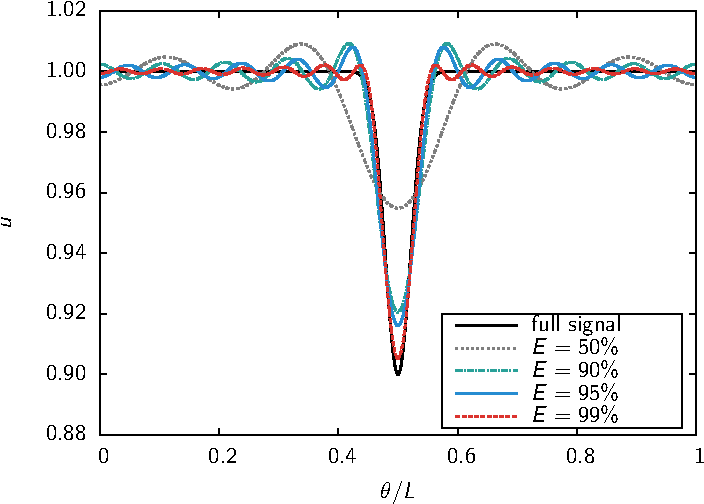
\includegraphics[width=.5\textwidth]{LEVEL_OF_ENERGY_PAPER.pdf}
  \caption{Reconstructions of a wake depending on
  the energy content kept in the signal.}
  \label{fig:level_of_energy}
\end{figure}
One can see
that a reconstruction using only 50\% of the energy
leads to a signal that has neither
the right wake deficit nor the correct width. Using
90\% and 95\% of the energy improve the resulting shape
but  large secondary
oscillations remain, with a bad capture
of the wake deficit.
In opposite, by using 99\% of the energy to reconstruct
the signal, only minor
oscillations are seen but 
the wake width and deficit are recovered with more than 
95\% accuracy.
Thus, the 99\% energy threshold ensures that the wake
will be correctly transmitted to the opposite row, which is
the prior concern of this Section.

To have a global insight of the energy contained in the
tangential distortion across the whole span,
the energy accumulation is plotted using a color map
in Fig.~\ref{fig:DREAM_LS_RANS_ROE2_SPECTRUM_PPT}.
Three contour lines are added to ease the
interpretation: 90\%, 95\%
and 99\% of accumulated energy, corresponding to a truncation
error of respectively 30\%, 20\% and 10\%.
Four harmonics are needed to capture 99\% of the energy, even though
at a relative span superior to 60\%, only three harmonics would be needed.
However, as the implementation of the harmonic balance used
in this work does not allow a varying number of harmonics through the
configuration, four harmonics is supposed to be sufficient to efficiently 
represent the unsteady flow field.
\begin{figure}[htp]
  \centering
  \includegraphics*[width=0.5\textwidth]{DREAM_LS_RANS_ROE2_SPECTRUM_PPT.pdf}
  \caption{Low-speed isolated configuration: prediction of the number
  of harmonics needed to simulate the configuration.}
  \label{fig:DREAM_LS_RANS_ROE2_SPECTRUM_PPT}
\end{figure}

\subsection{Analyzing the similarity coefficients}
\label{sub:dream_ls_conv_hb_sim_coeff}
To confirm the number of harmonics needed to ensure the convergence
of harmonic balance computations, simulations are run with up to four
harmonics. The strategy used to launch the computation is as follow:
the steady computation is used as an initial guess for the $N=1$ HB computation.
Then each new HB computation is launched with the previous one as initial
solution.

Two harmonics are actually necessary to converge the temporal mean 
of the similarity coefficients as show 
in Tab.~\ref{tab:dream_ls_hb_conv_sim}. After that, a slight evolution of the
coefficients is still seen but represents a change lower than 0.01\%
of the $N=4$ results, hence the convergence. 
\begin{table}[htp]
  \ra{1.3} \centering
  \begin{tabular}{rccccc}
    \toprule
    & steady & HB $N=1$ & HB $N=2$ & HB $N=3$ & HB $N=4$ \\
    \midrule
    $C_T$  & $1.1319$ & $1.1334$ & $1.1330$ & $1.1330$ & $1.1329$ \\
    $C_P$  & $2.0927$ & $2.0951$ & $2.0944$ & $2.0945$ & $2.0946$ \\
    $\eta$ & $0.5726$ & $0.5727$ & $0.5726$ & $0.5726$ & $0.5725$ \\
    \bottomrule
  \end{tabular}
  \caption{Low-speed isolated configuration: analysis of the number of harmonics
  required to capture the mean similarity coefficients.}
  \label{tab:dream_ls_hb_conv_sim}
\end{table}
Note that a steady computation is sufficient to retrieve
the temporal mean value of the similarity coefficients.
In fact, on this variables, a maximum of 0.1\% difference is observed by
comparing the mixing plane and harmonic balance results.

\subsection{Analyzing the blade response}
\label{sub:dream_ls_conv_hb_blade_response}
Of course, analyzing integrated results to assess the converge of
a computation is a primarily step that should be complemented with
a local analysis. In this way, a discrete Fourier transform is
performed to analyze the first harmonic of the static pressure on the 
rear rotor blades. Due to the passing
of the front rotor wakes, these blades will experience a
high level of unsteadinesses. It is therefore considered as a
bottleneck in the convergence of the HB computations, hence its analysis.
The results are shown in 
Fig.~\ref{fig:dream_ls_hb_blade_response_conv}. 
\begin{figure}[htp]
 \ra{1.3} \centering
 \begin{tabular}{r|cccc}
   \toprule
   & \multicolumn{2}{c}{mean} & \multicolumn{2}{c}{1\textsuperscript{st} harmonic} \\
   & \multicolumn{2}{c}{
        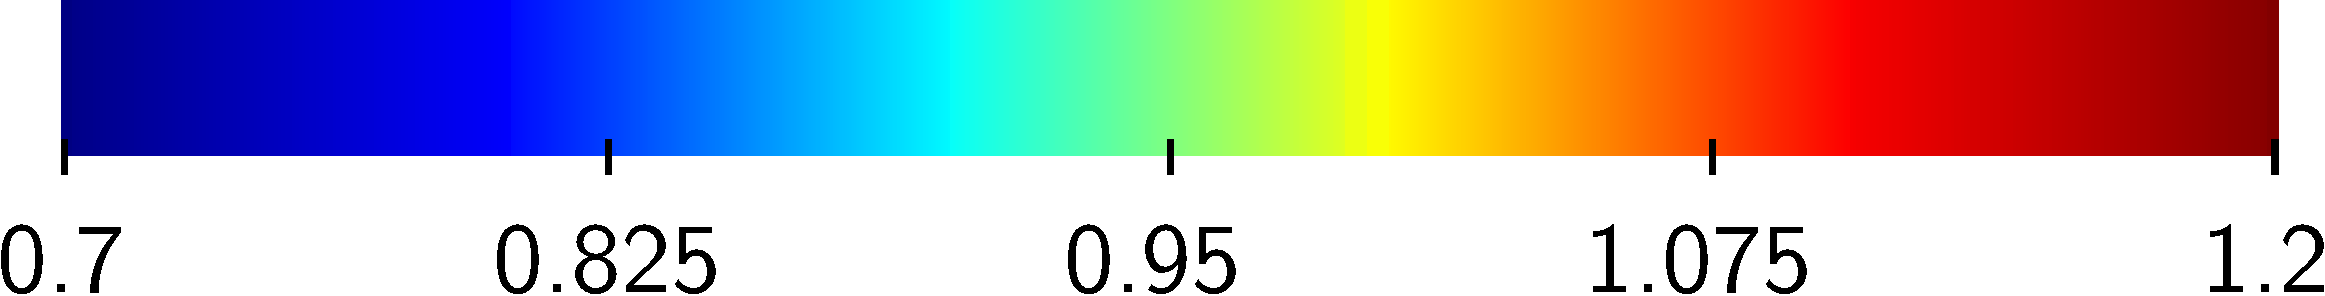
\includegraphics[width=0.22\textwidth]{dream_ls_blade_resp_scale_mean.pdf}} 
   & \multicolumn{2}{c}{
        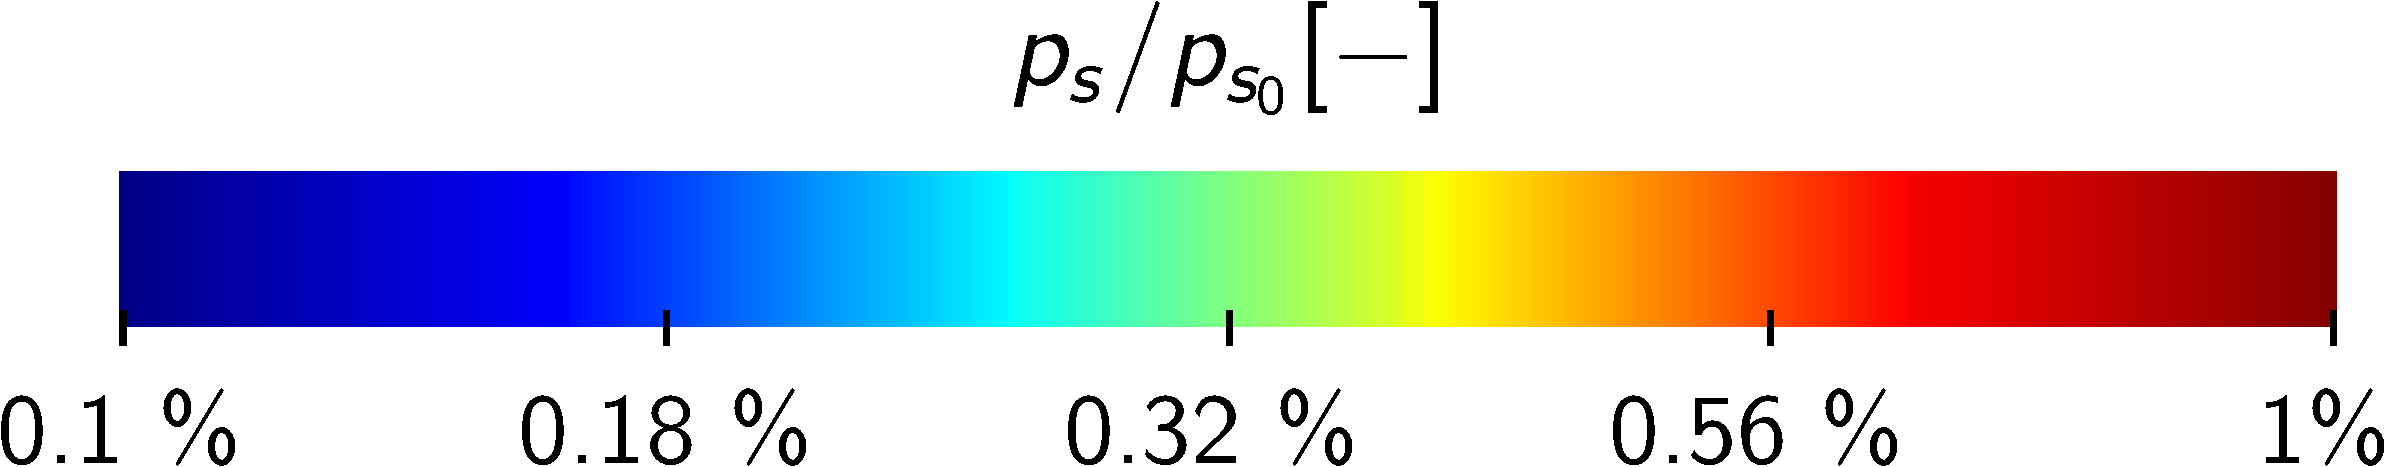
\includegraphics[width=0.22\textwidth]{dream_ls_blade_resp_scale_H01_rear.pdf}} \\
   \midrule
   \rotatebox{90}{\quad\quad\quad steady} 
   & 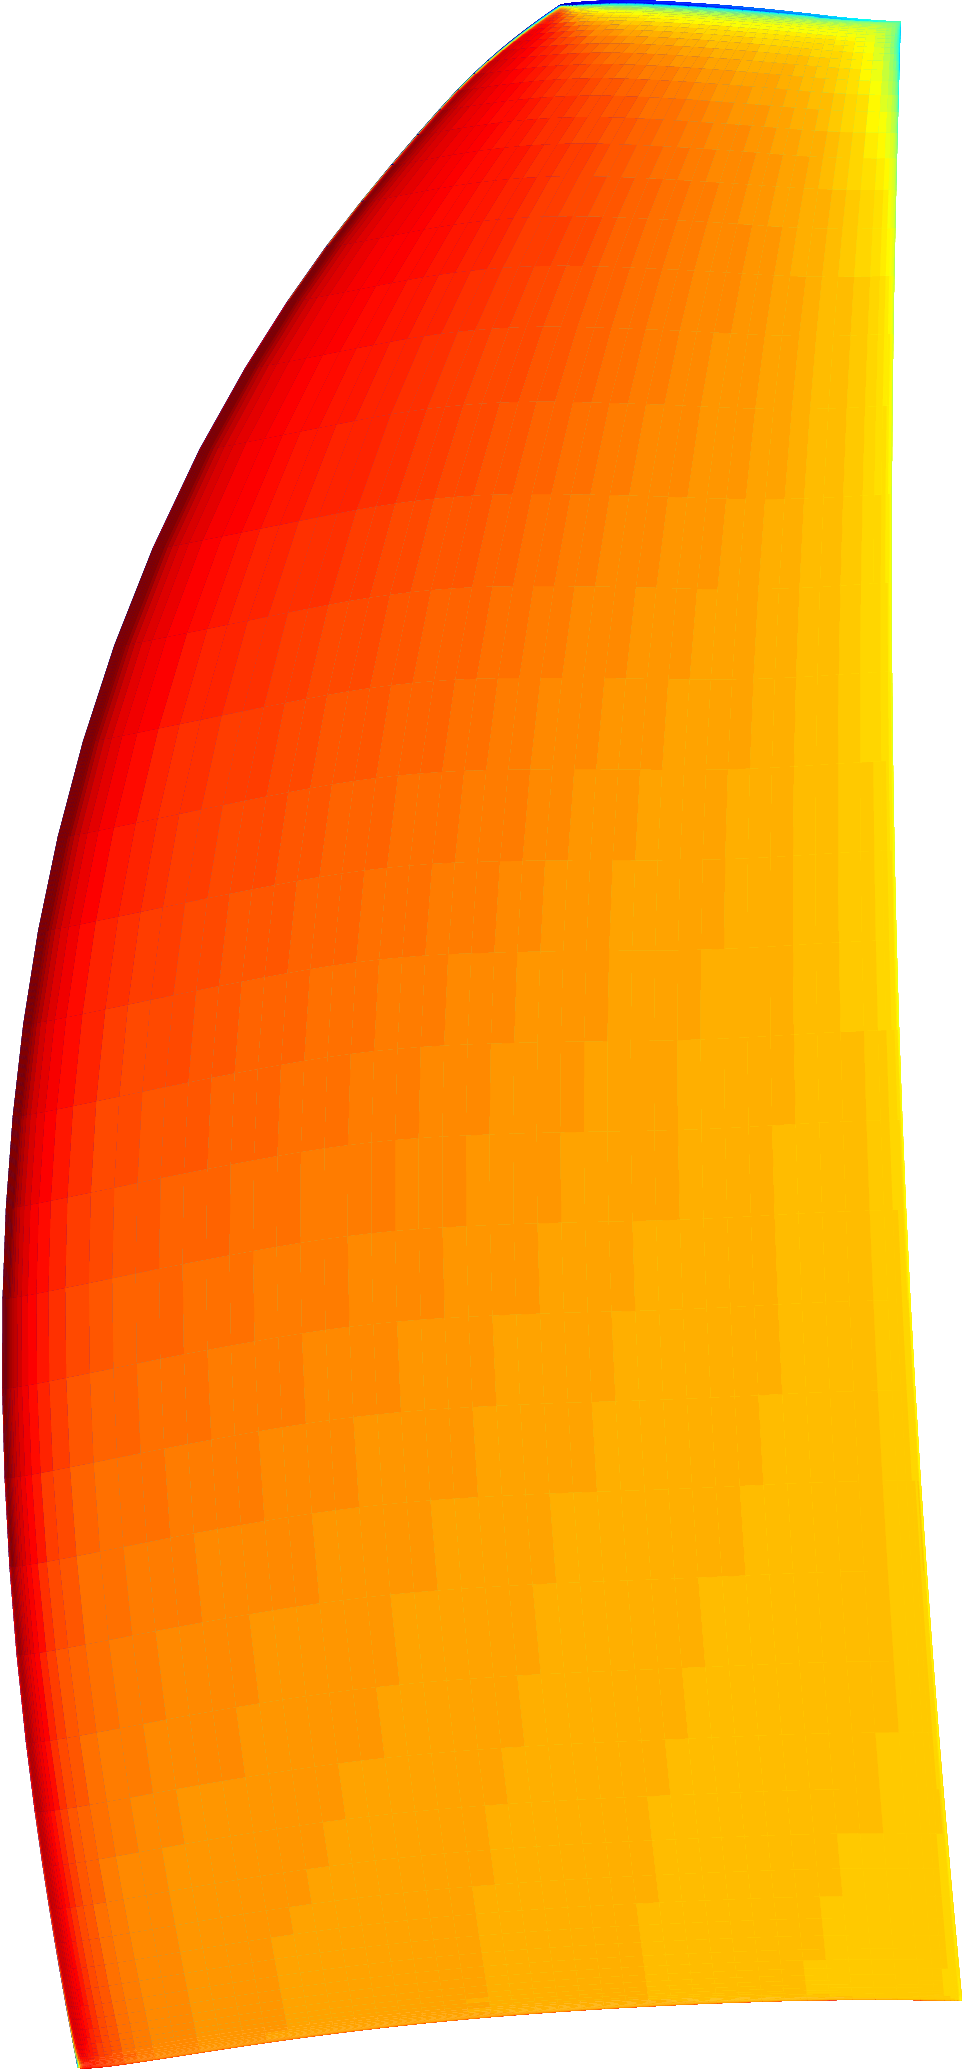
\includegraphics[width=0.10\textwidth]{DREAM_LS_RANS_roe2_sa_blade_response_rear_PS.png}
   & 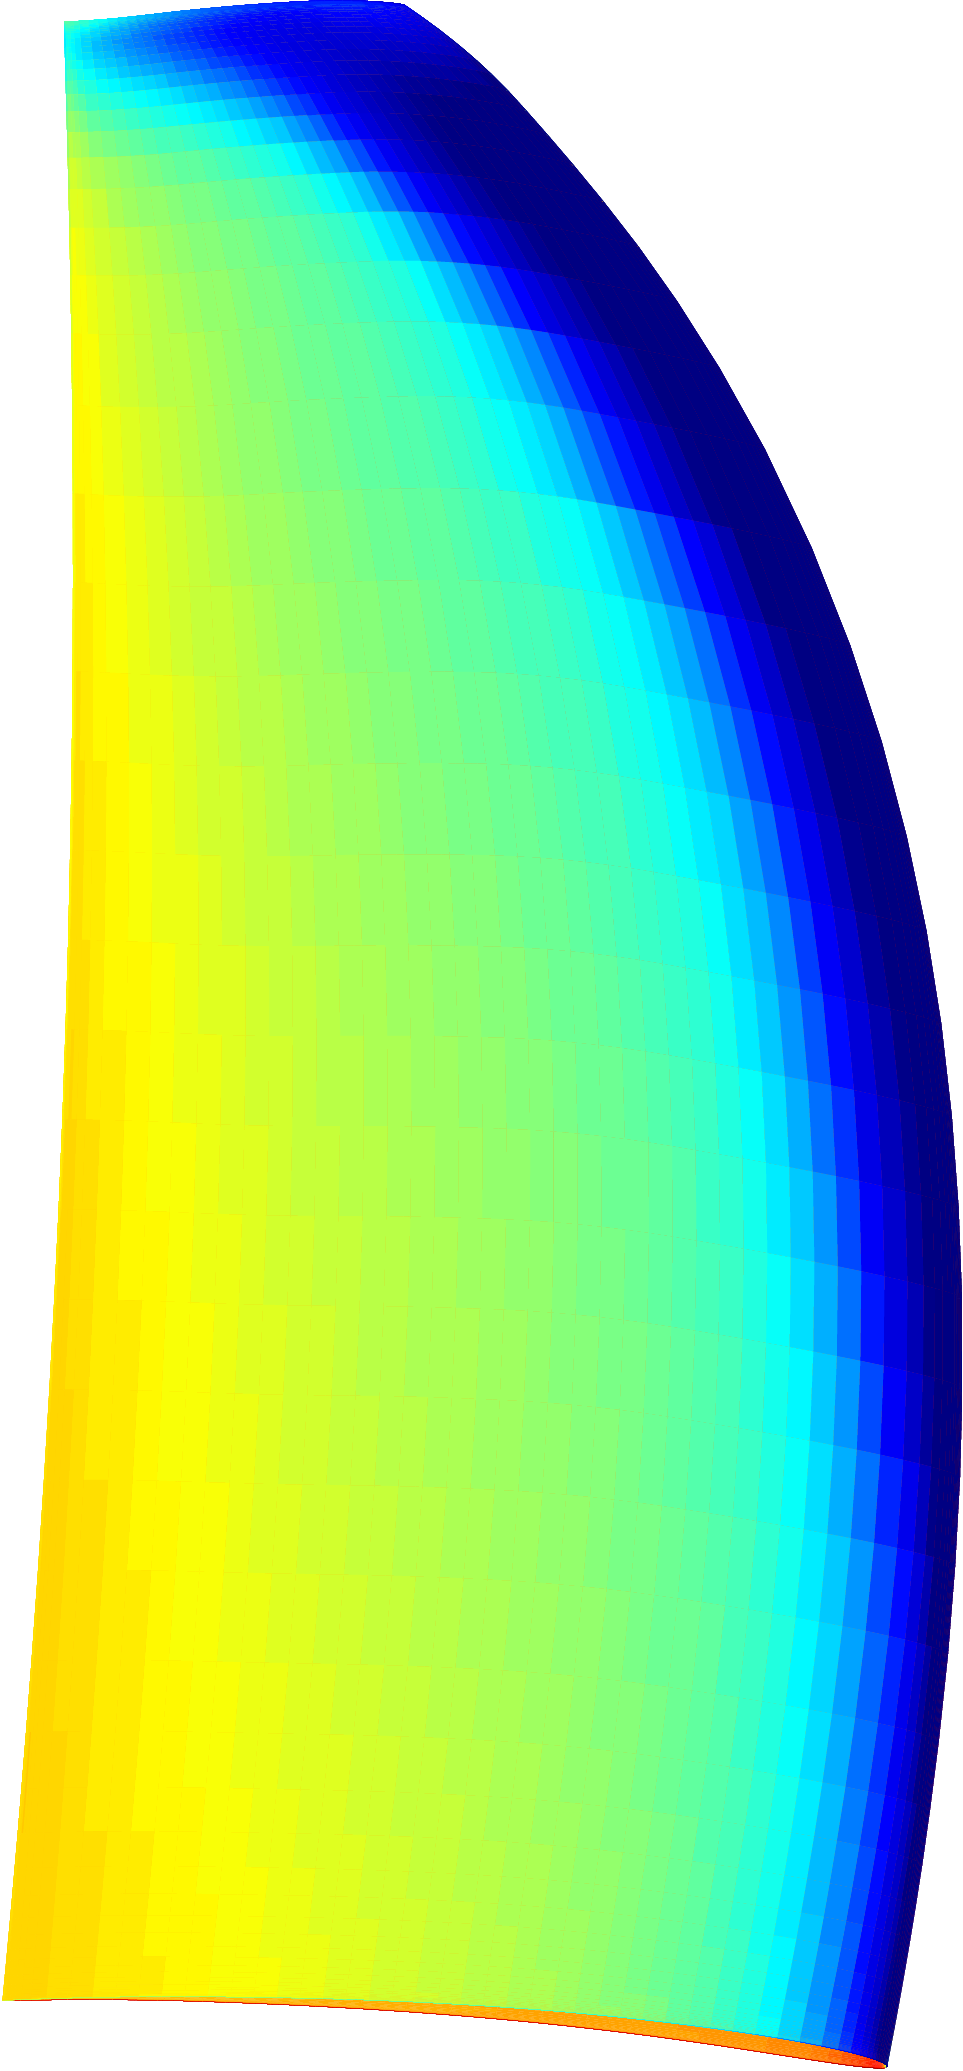
\includegraphics[width=0.10\textwidth]{DREAM_LS_RANS_roe2_sa_blade_response_rear_SS.png}
   &   &\\
   \rotatebox{90}{\quad\quad HB $N=1$} 
   & 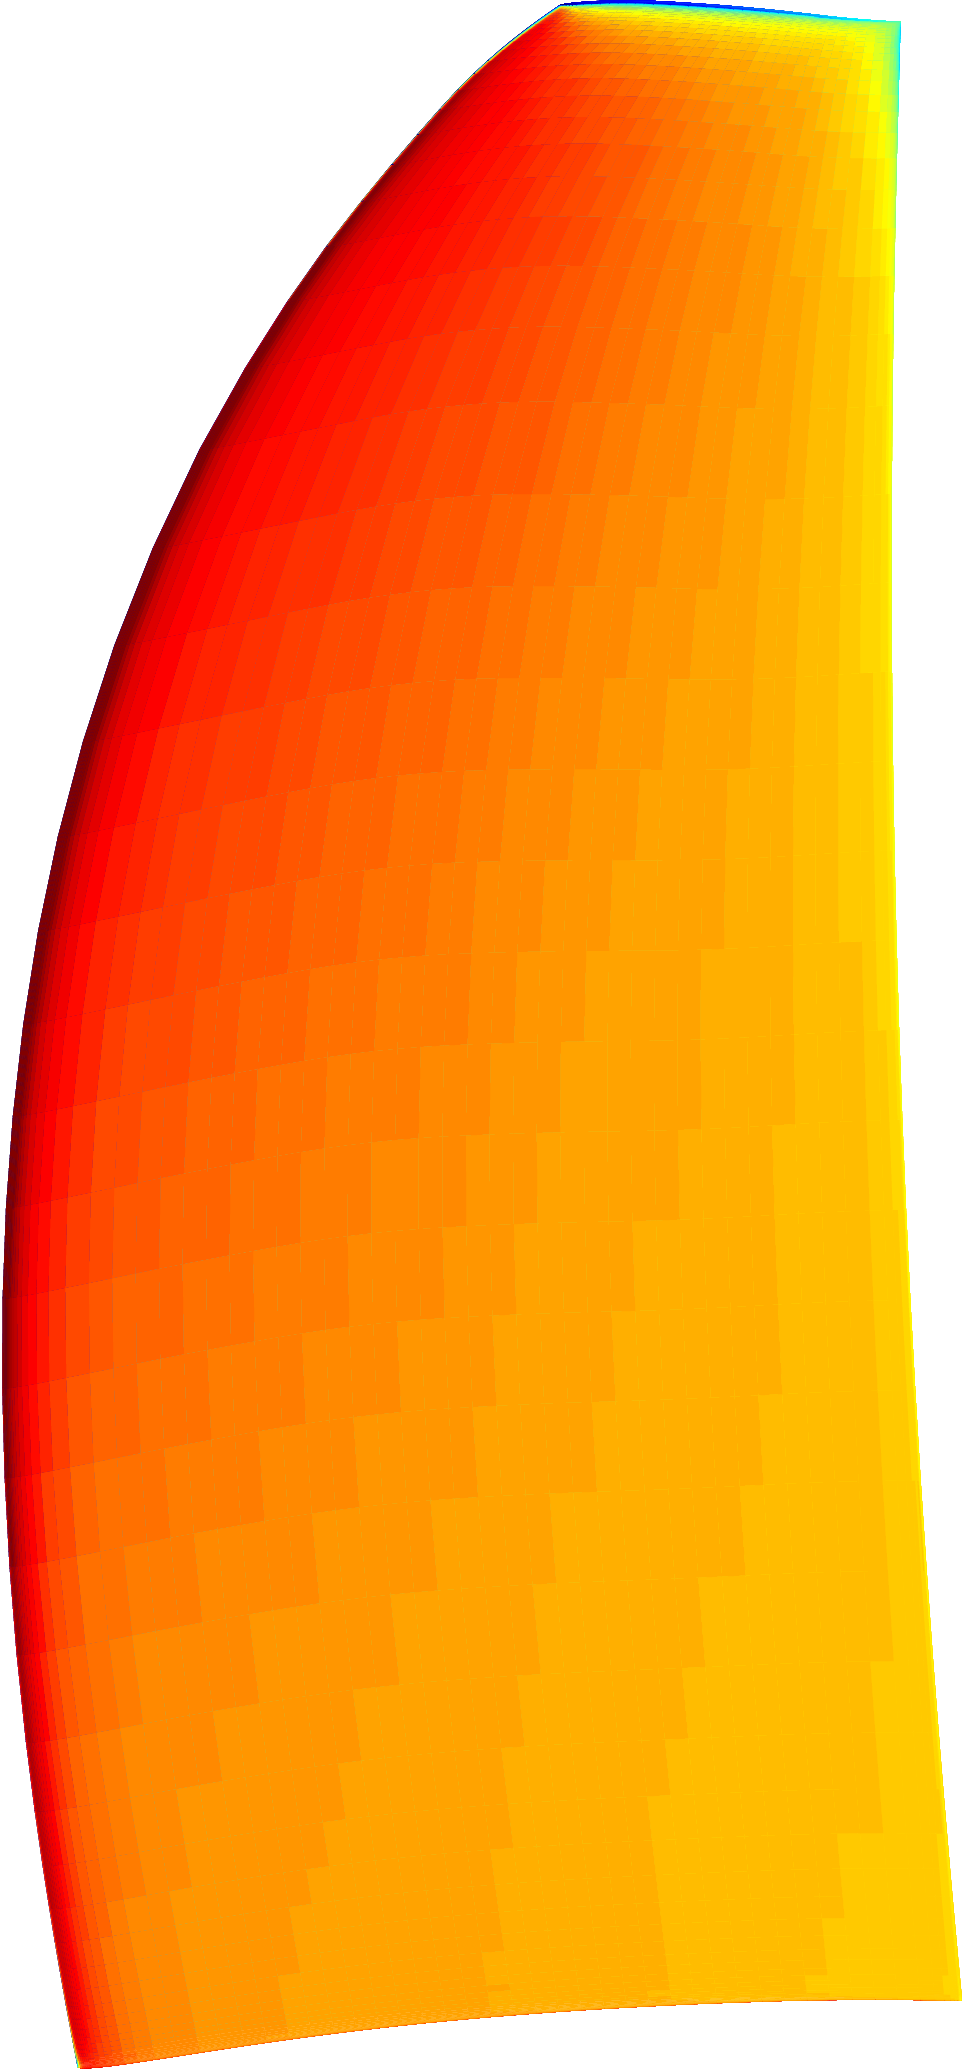
\includegraphics[width=0.10\textwidth]{DREAM_LS_TSM_N1_roe2_sa_blade_response_rear_mean_PS.png}
   & 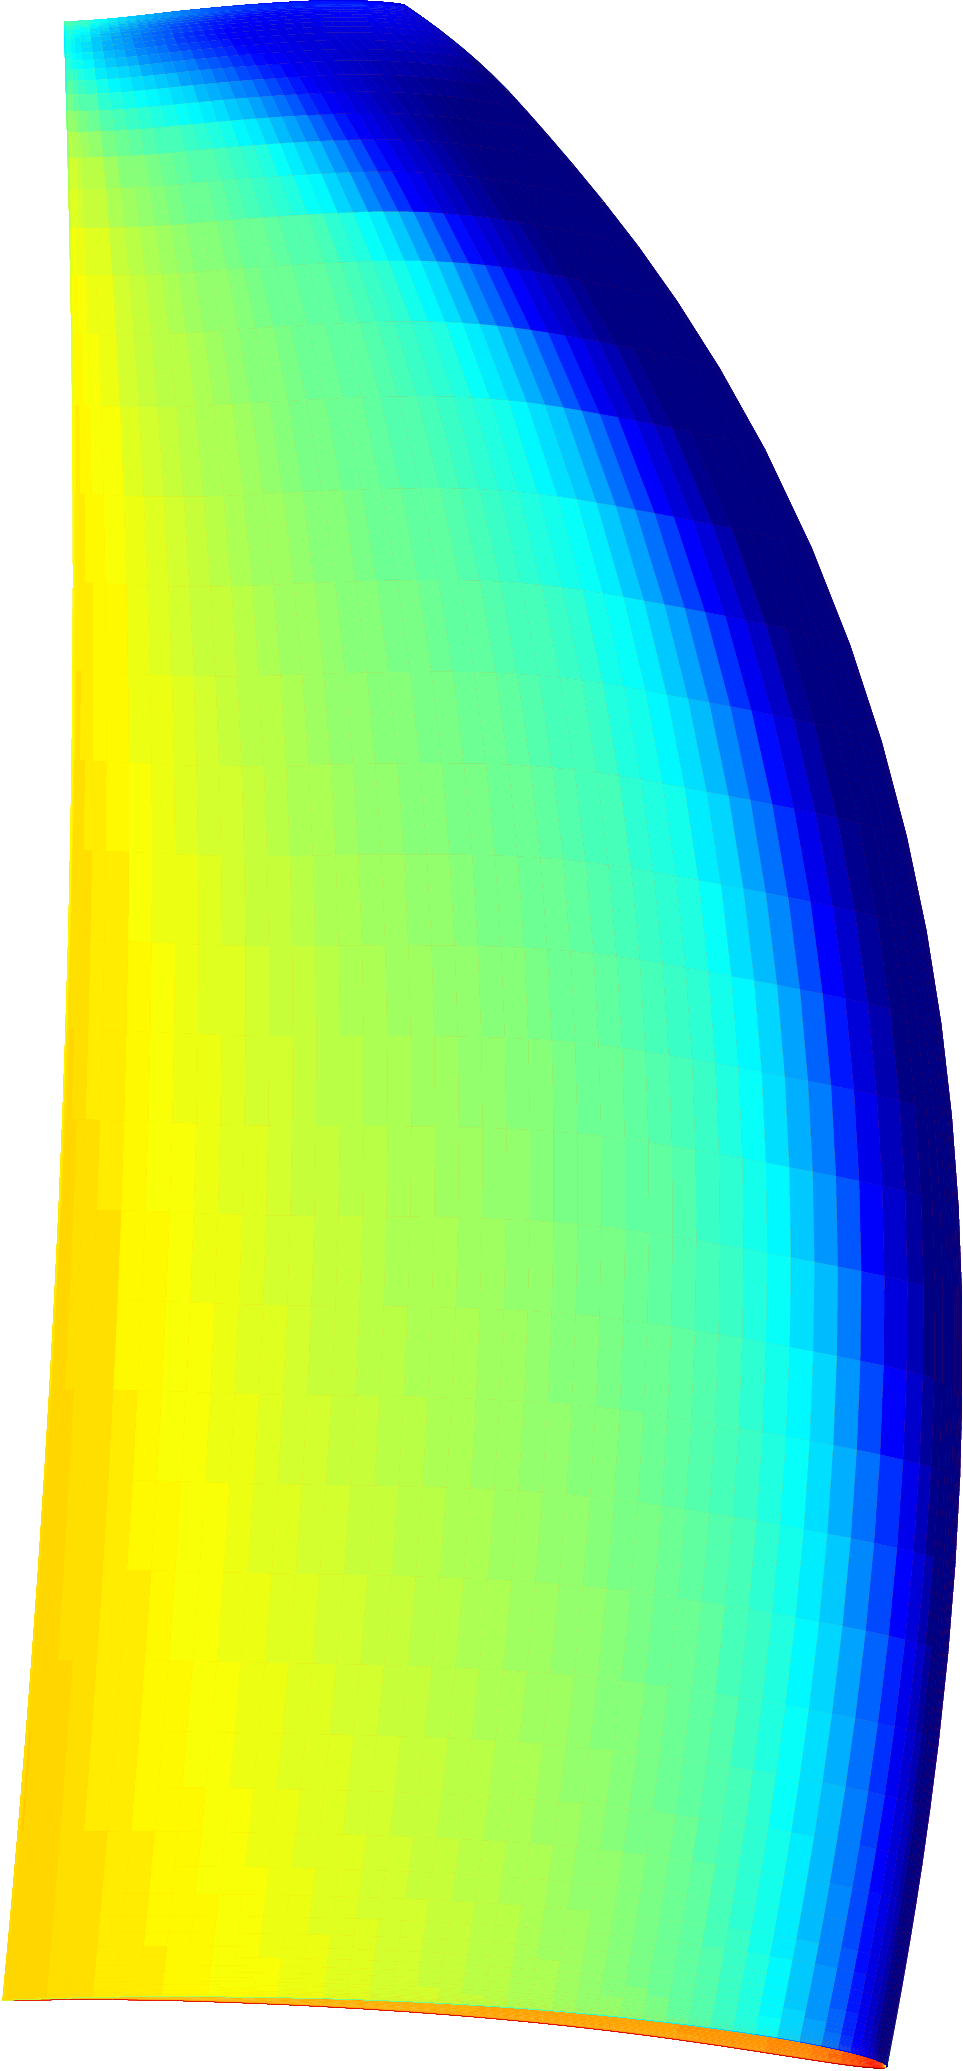
\includegraphics[width=0.10\textwidth]{DREAM_LS_TSM_N1_roe2_sa_blade_response_rear_mean_SS.png}
   & 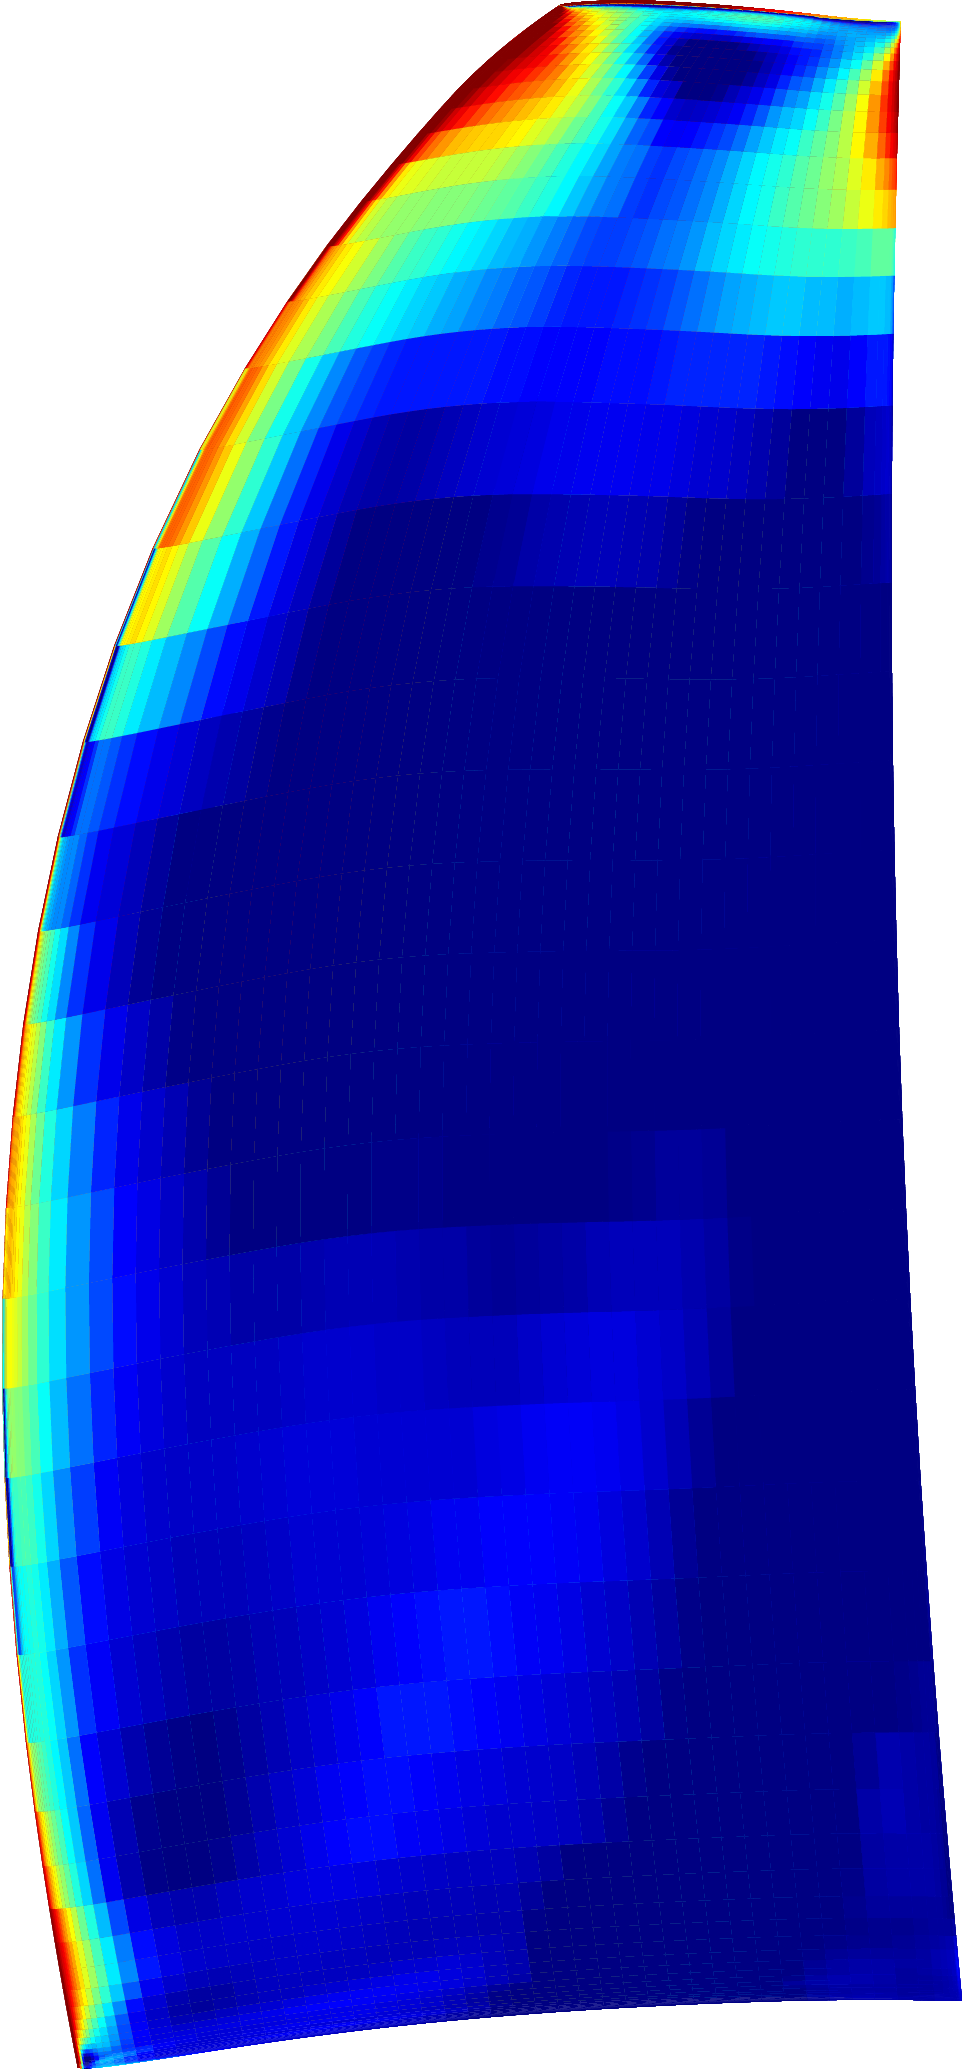
\includegraphics[width=0.10\textwidth]{DREAM_LS_TSM_N1_roe2_sa_blade_response_rear_H01_PS.png}
   & 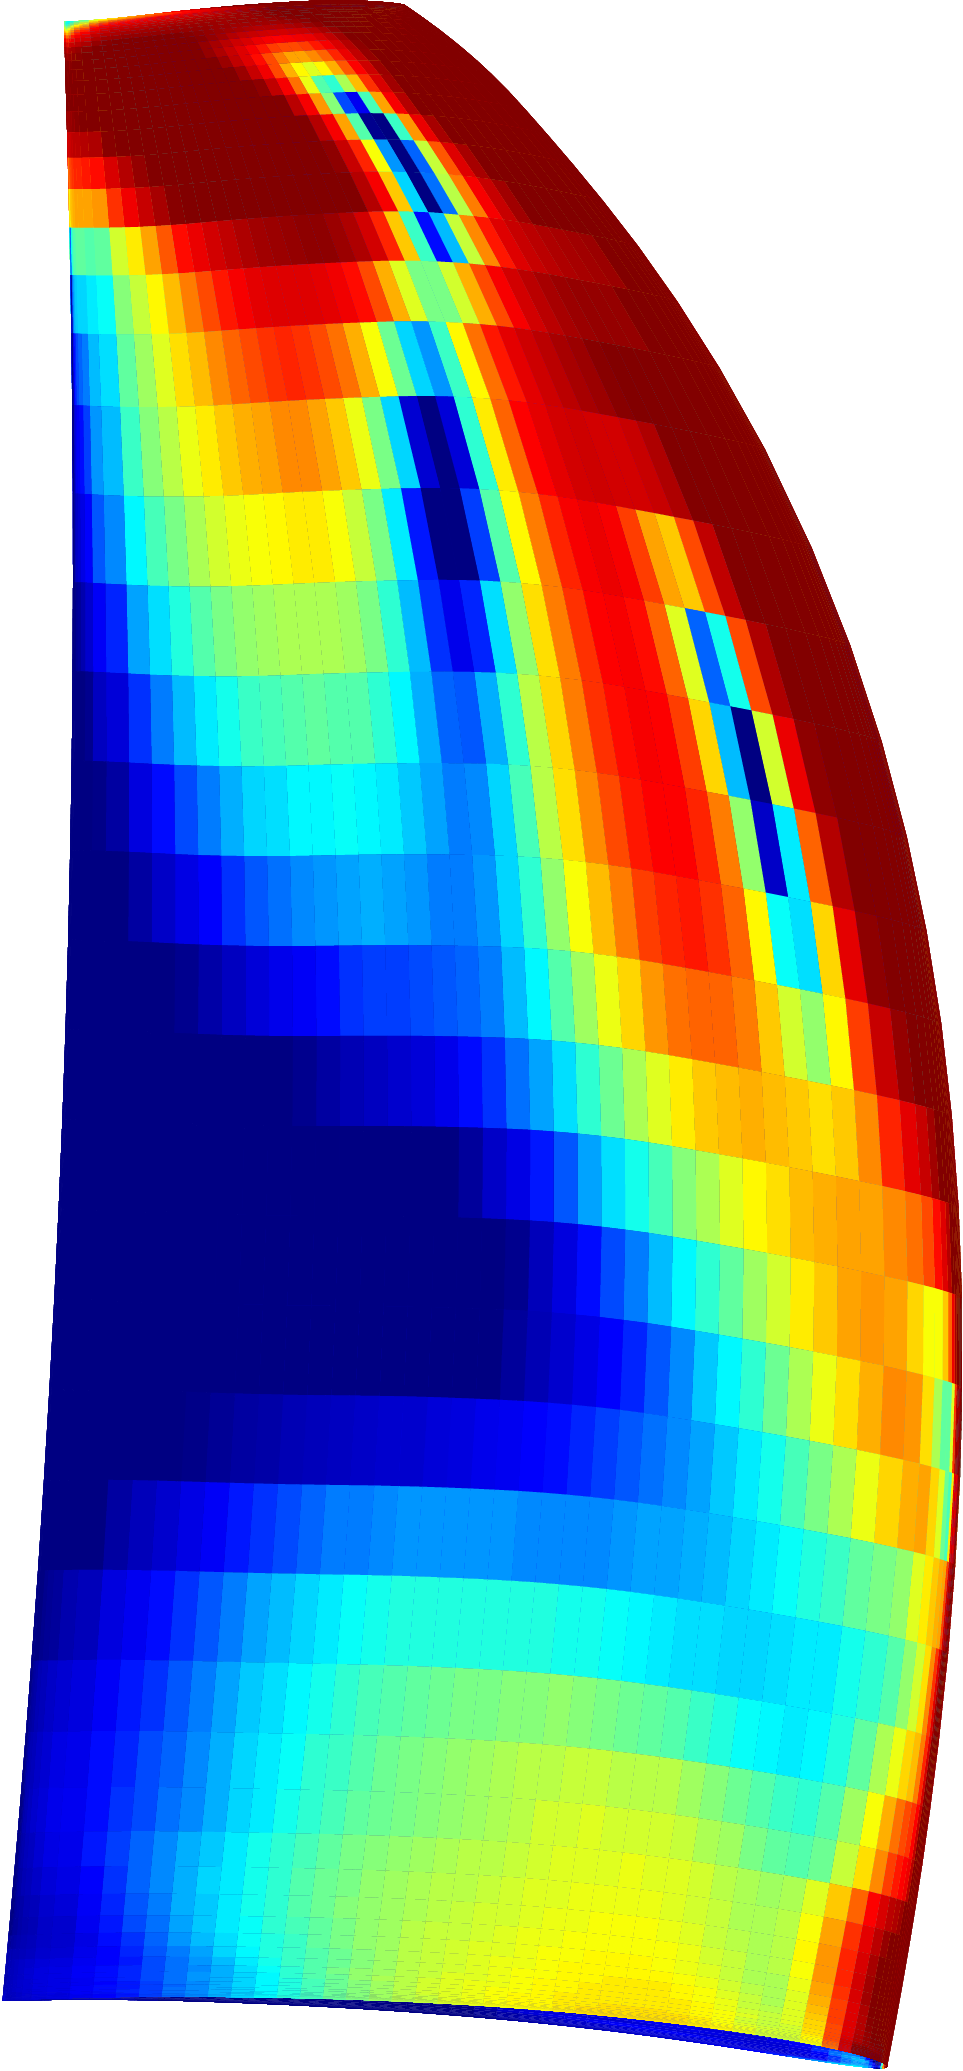
\includegraphics[width=0.10\textwidth]{DREAM_LS_TSM_N1_roe2_sa_blade_response_rear_H01_SS.png} \\
   \rotatebox{90}{\quad\quad HB $N=2$} 
   & 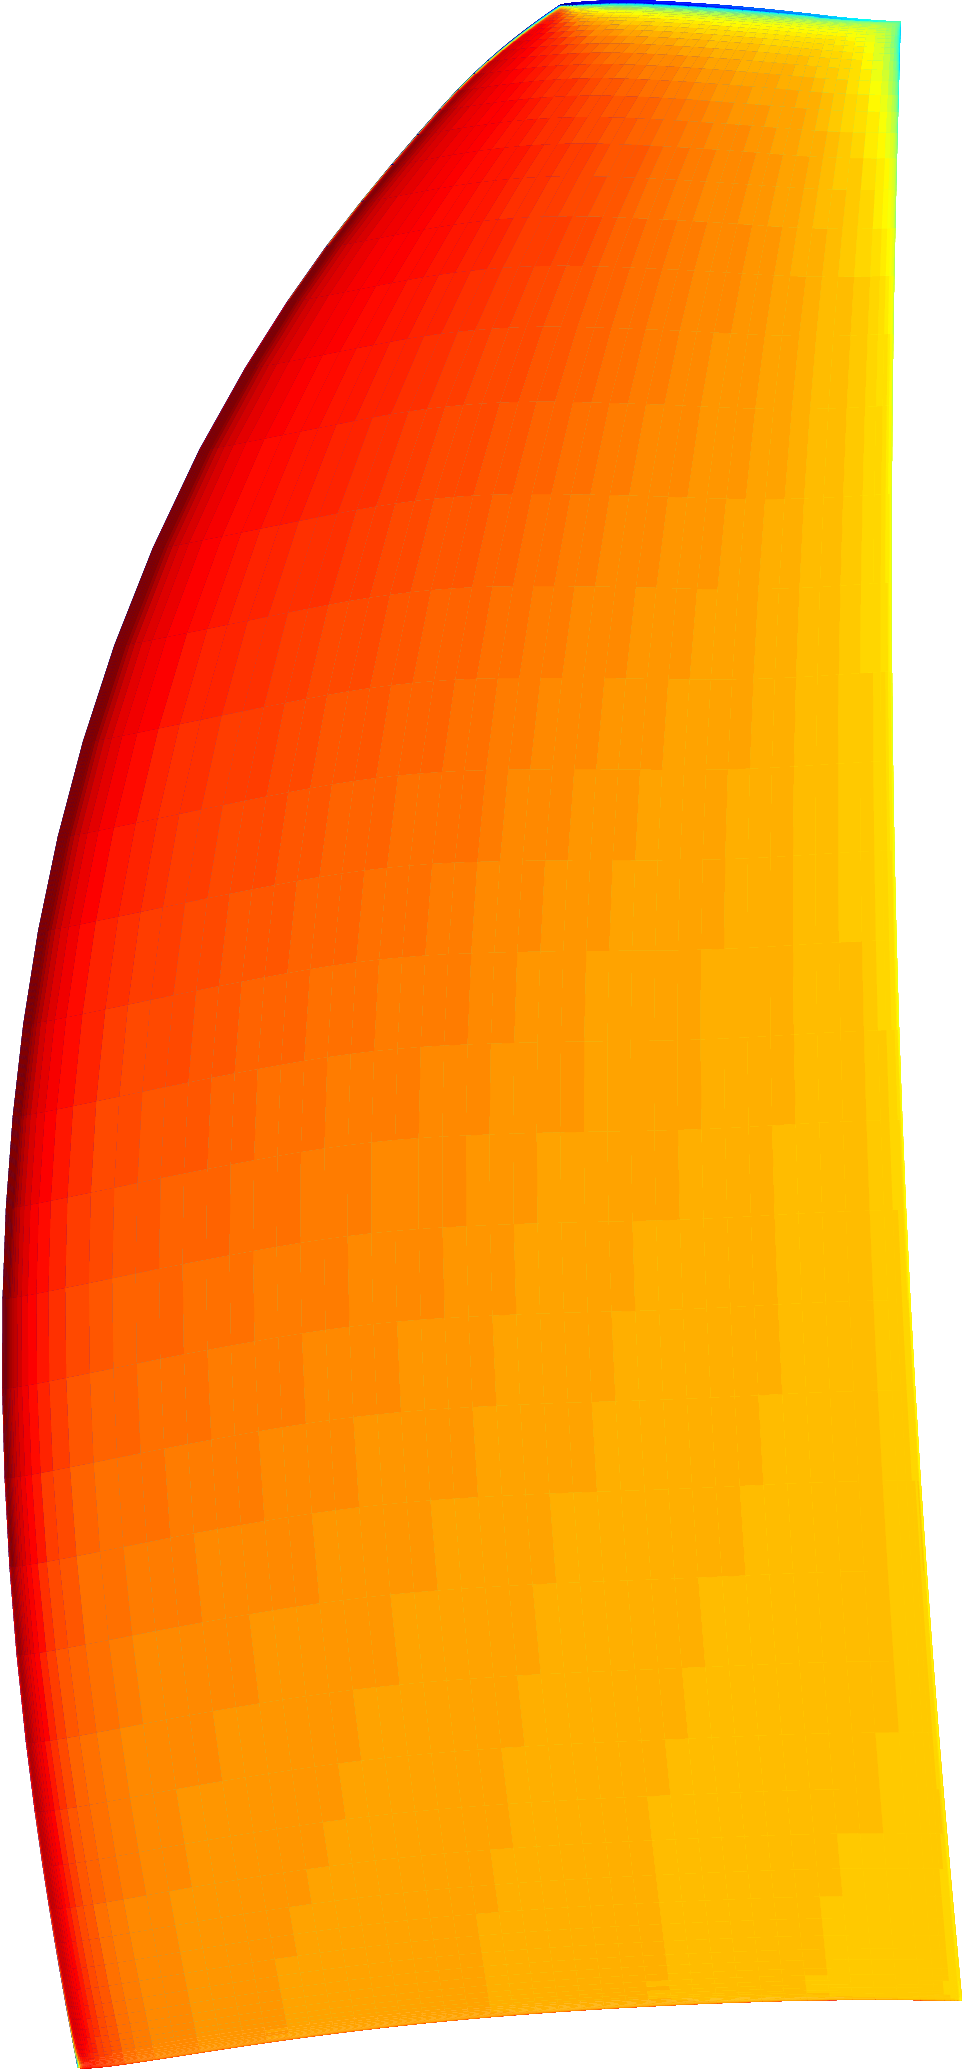
\includegraphics[width=0.10\textwidth]{DREAM_LS_TSM_N2_roe2_sa_blade_response_rear_mean_PS.png}
   & 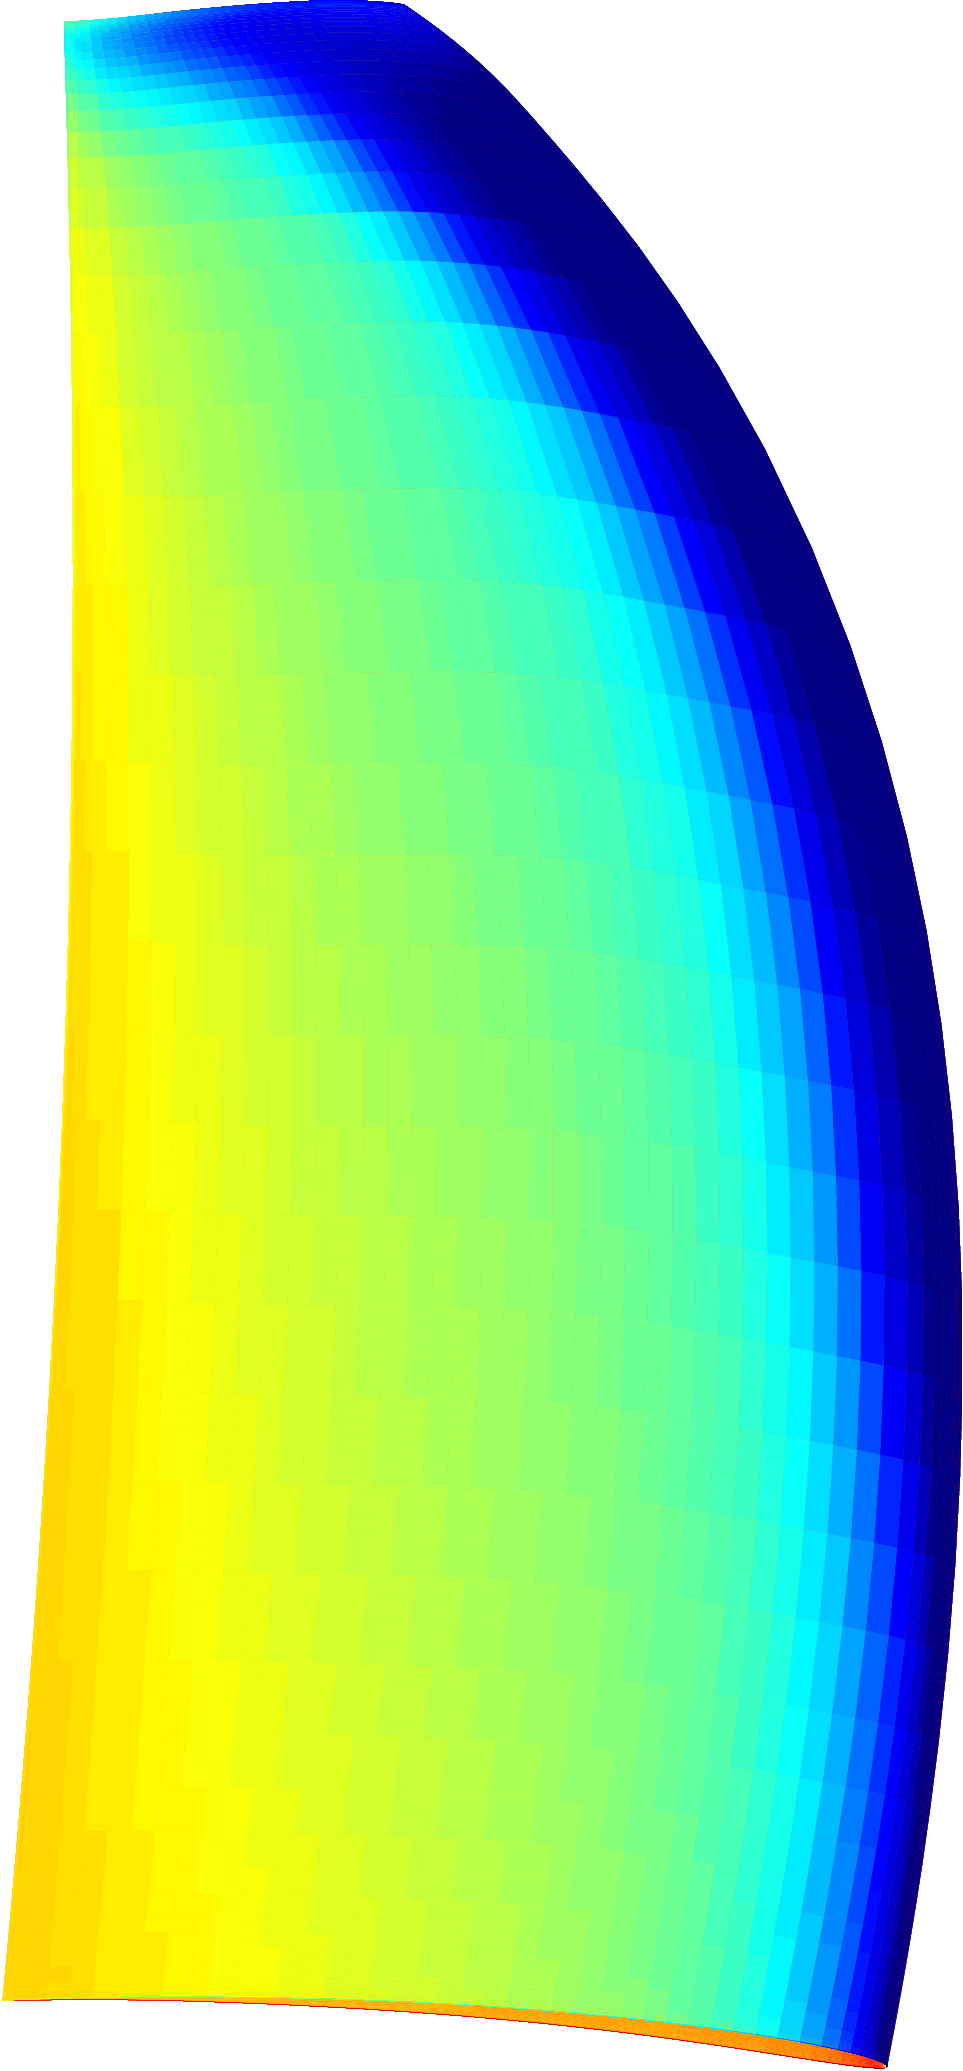
\includegraphics[width=0.10\textwidth]{DREAM_LS_TSM_N2_roe2_sa_blade_response_rear_mean_SS.png}
   & 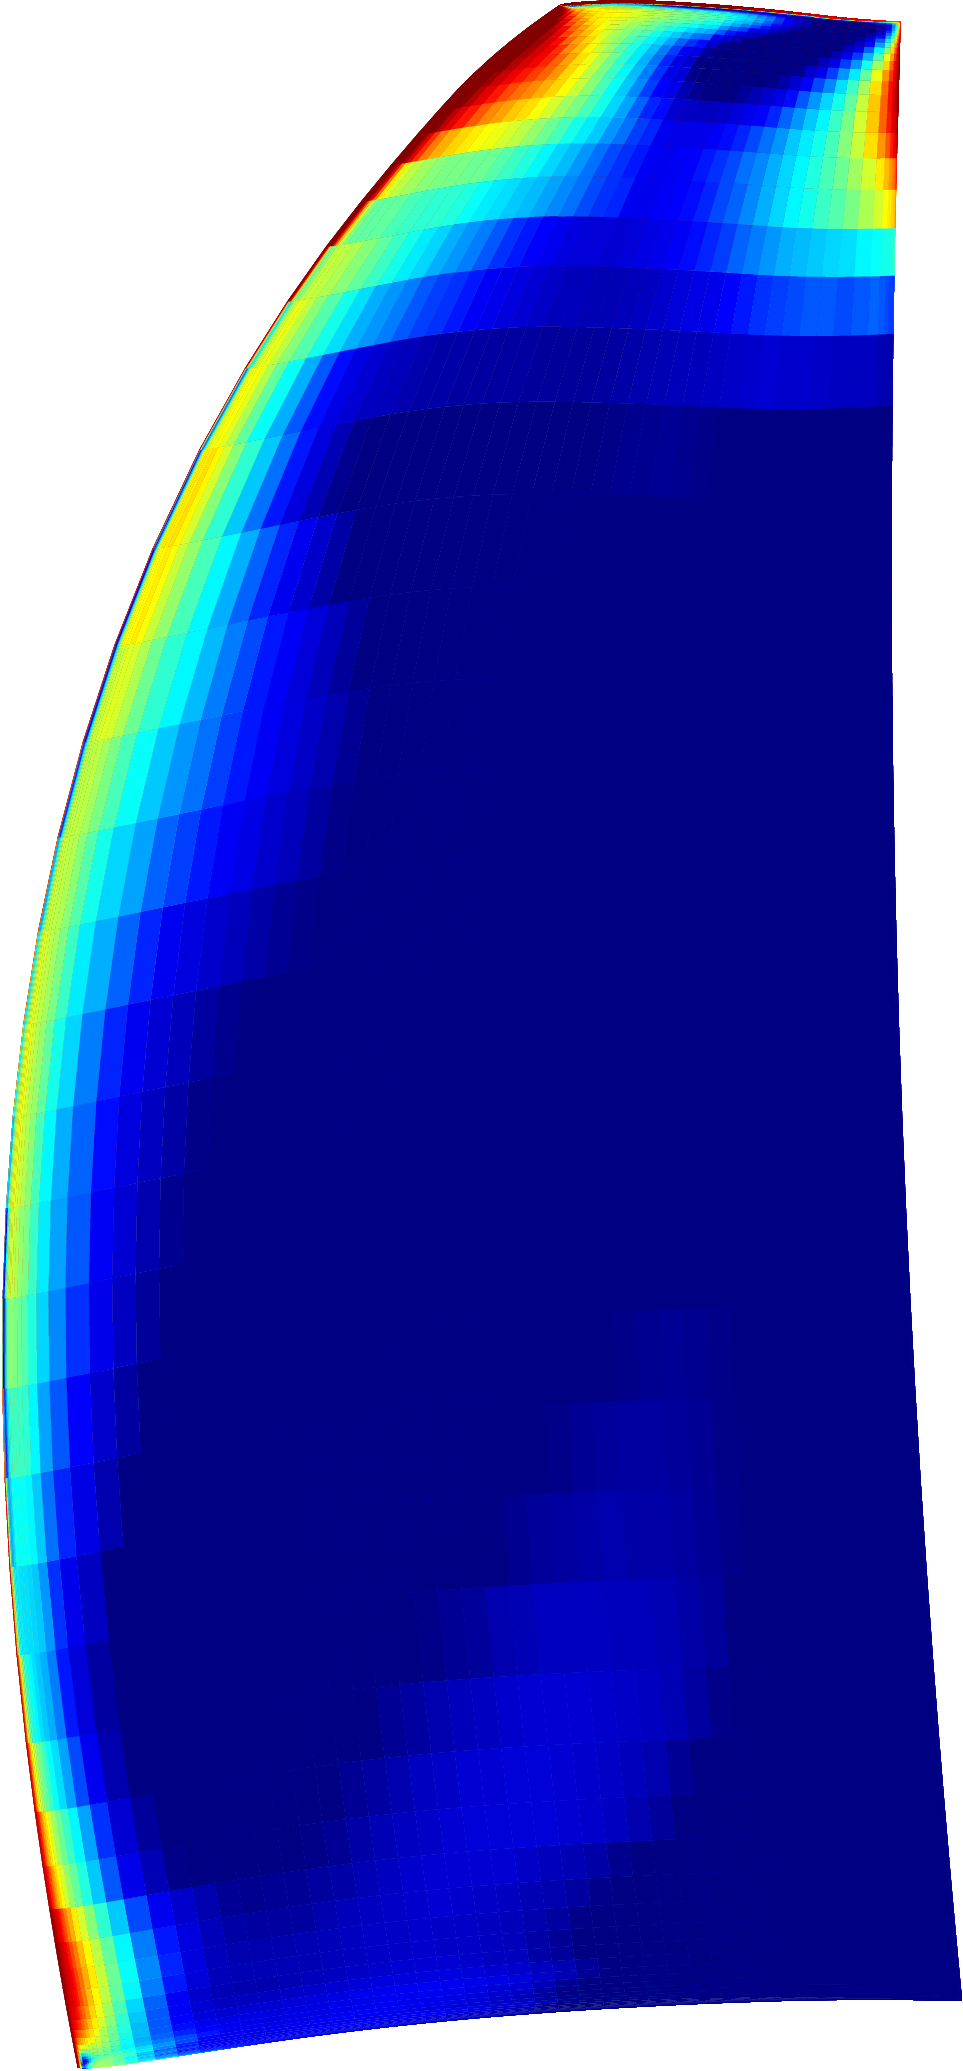
\includegraphics[width=0.10\textwidth]{DREAM_LS_TSM_N2_roe2_sa_blade_response_rear_H01_PS.png}
   & 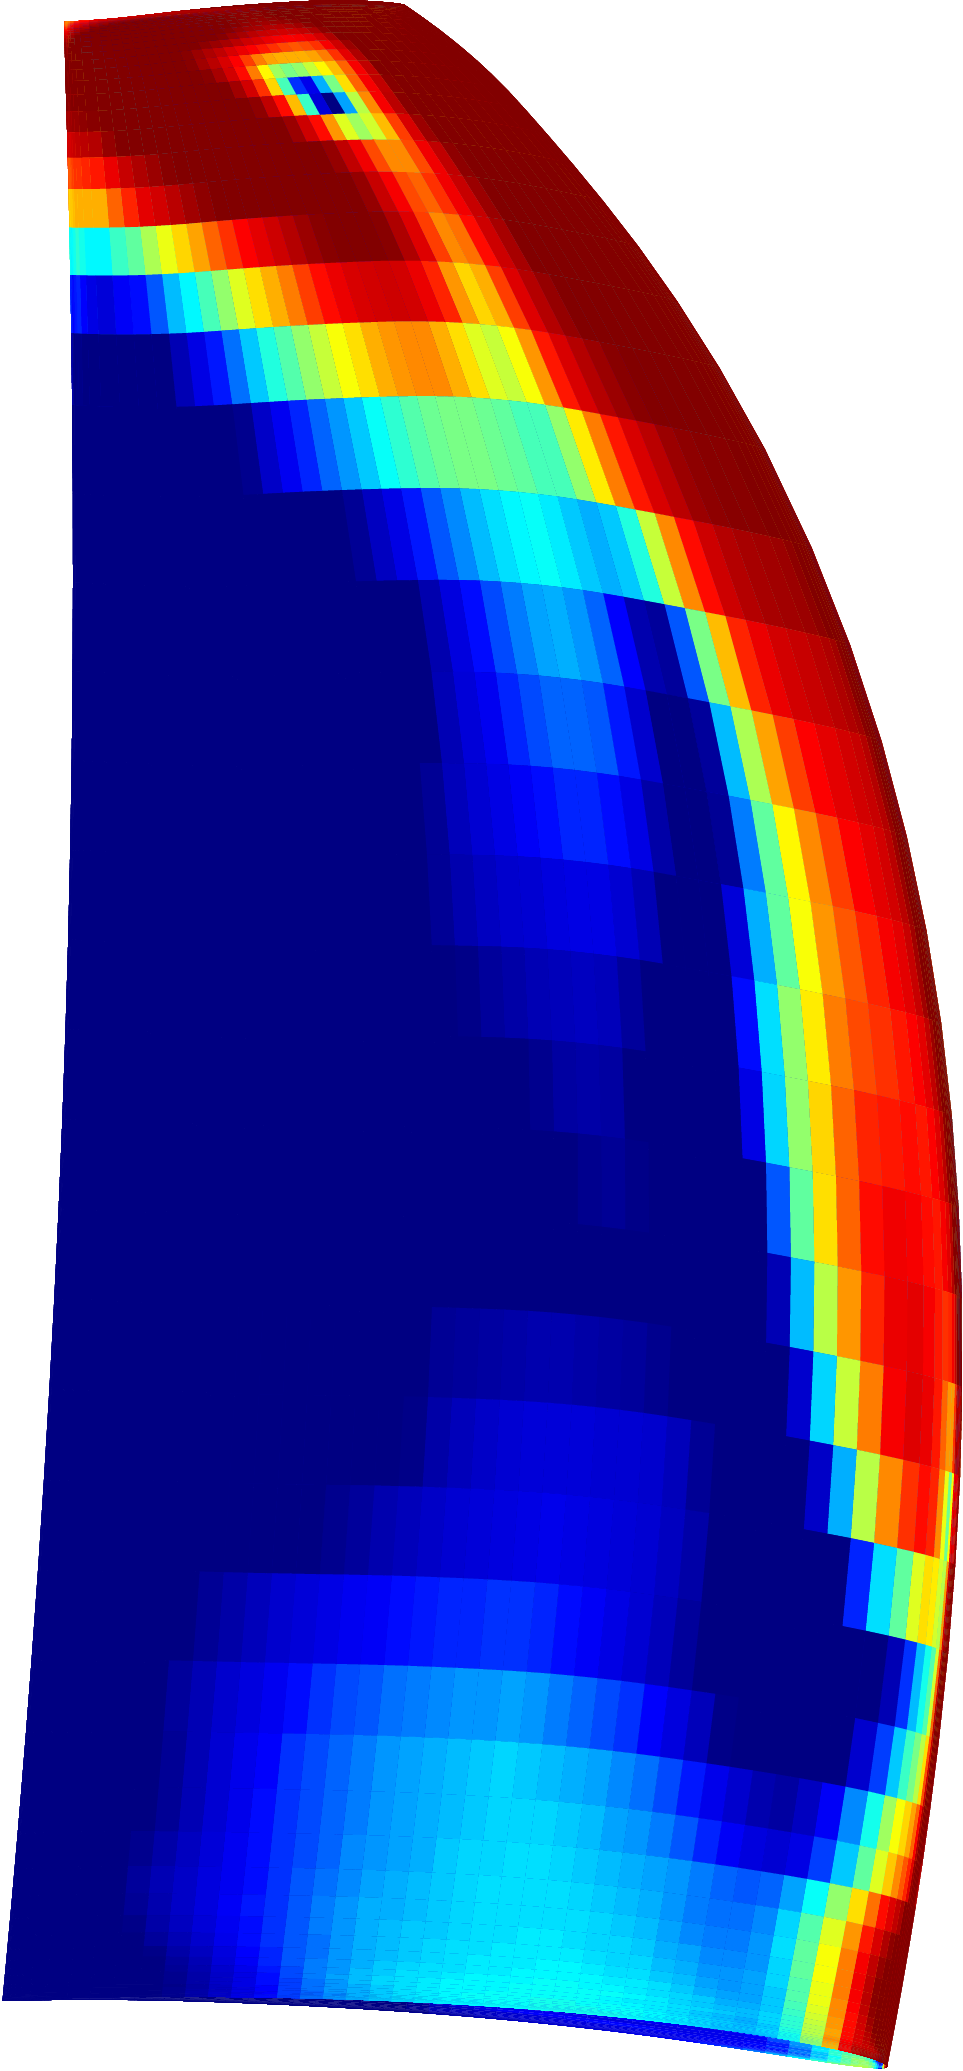
\includegraphics[width=0.10\textwidth]{DREAM_LS_TSM_N2_roe2_sa_blade_response_rear_H01_SS.png} \\
   \rotatebox{90}{\quad\quad HB $N=3$} 
   & 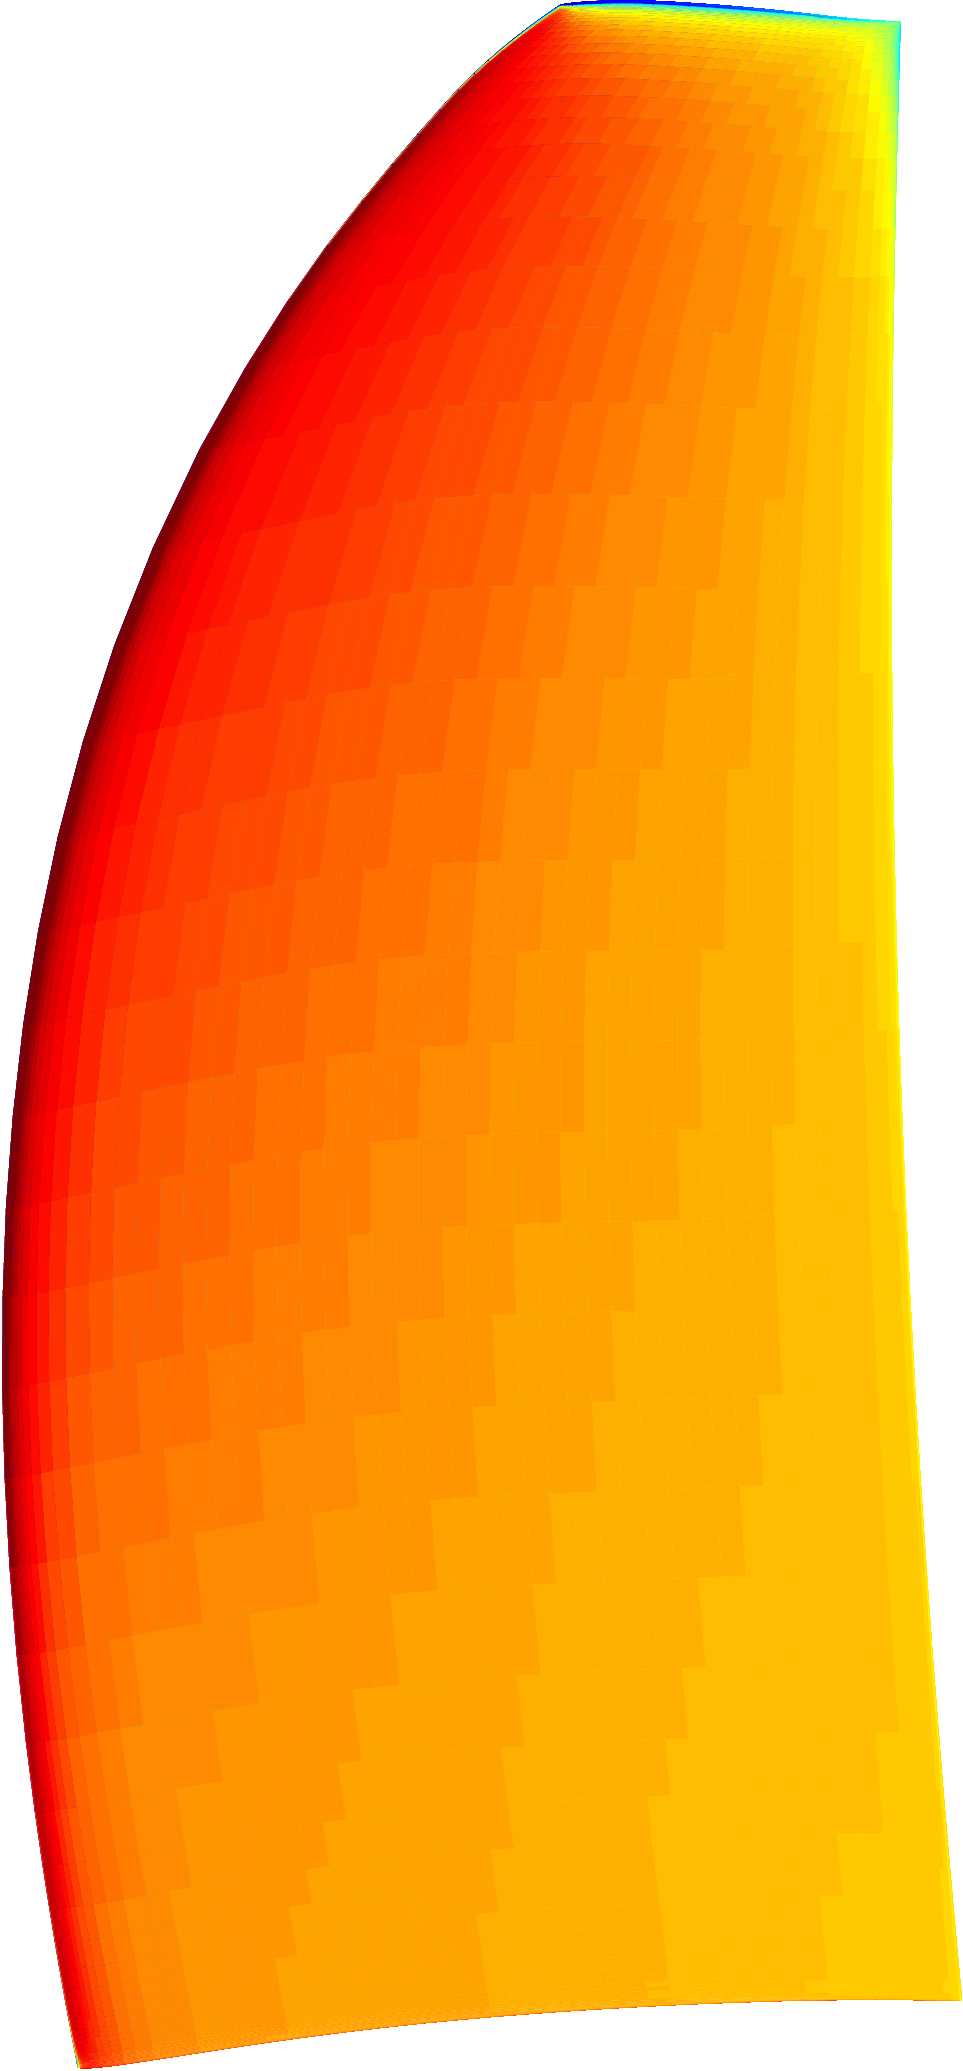
\includegraphics[width=0.10\textwidth]{DREAM_LS_TSM_N3_roe2_sa_blade_response_rear_mean_PS.png}
   & 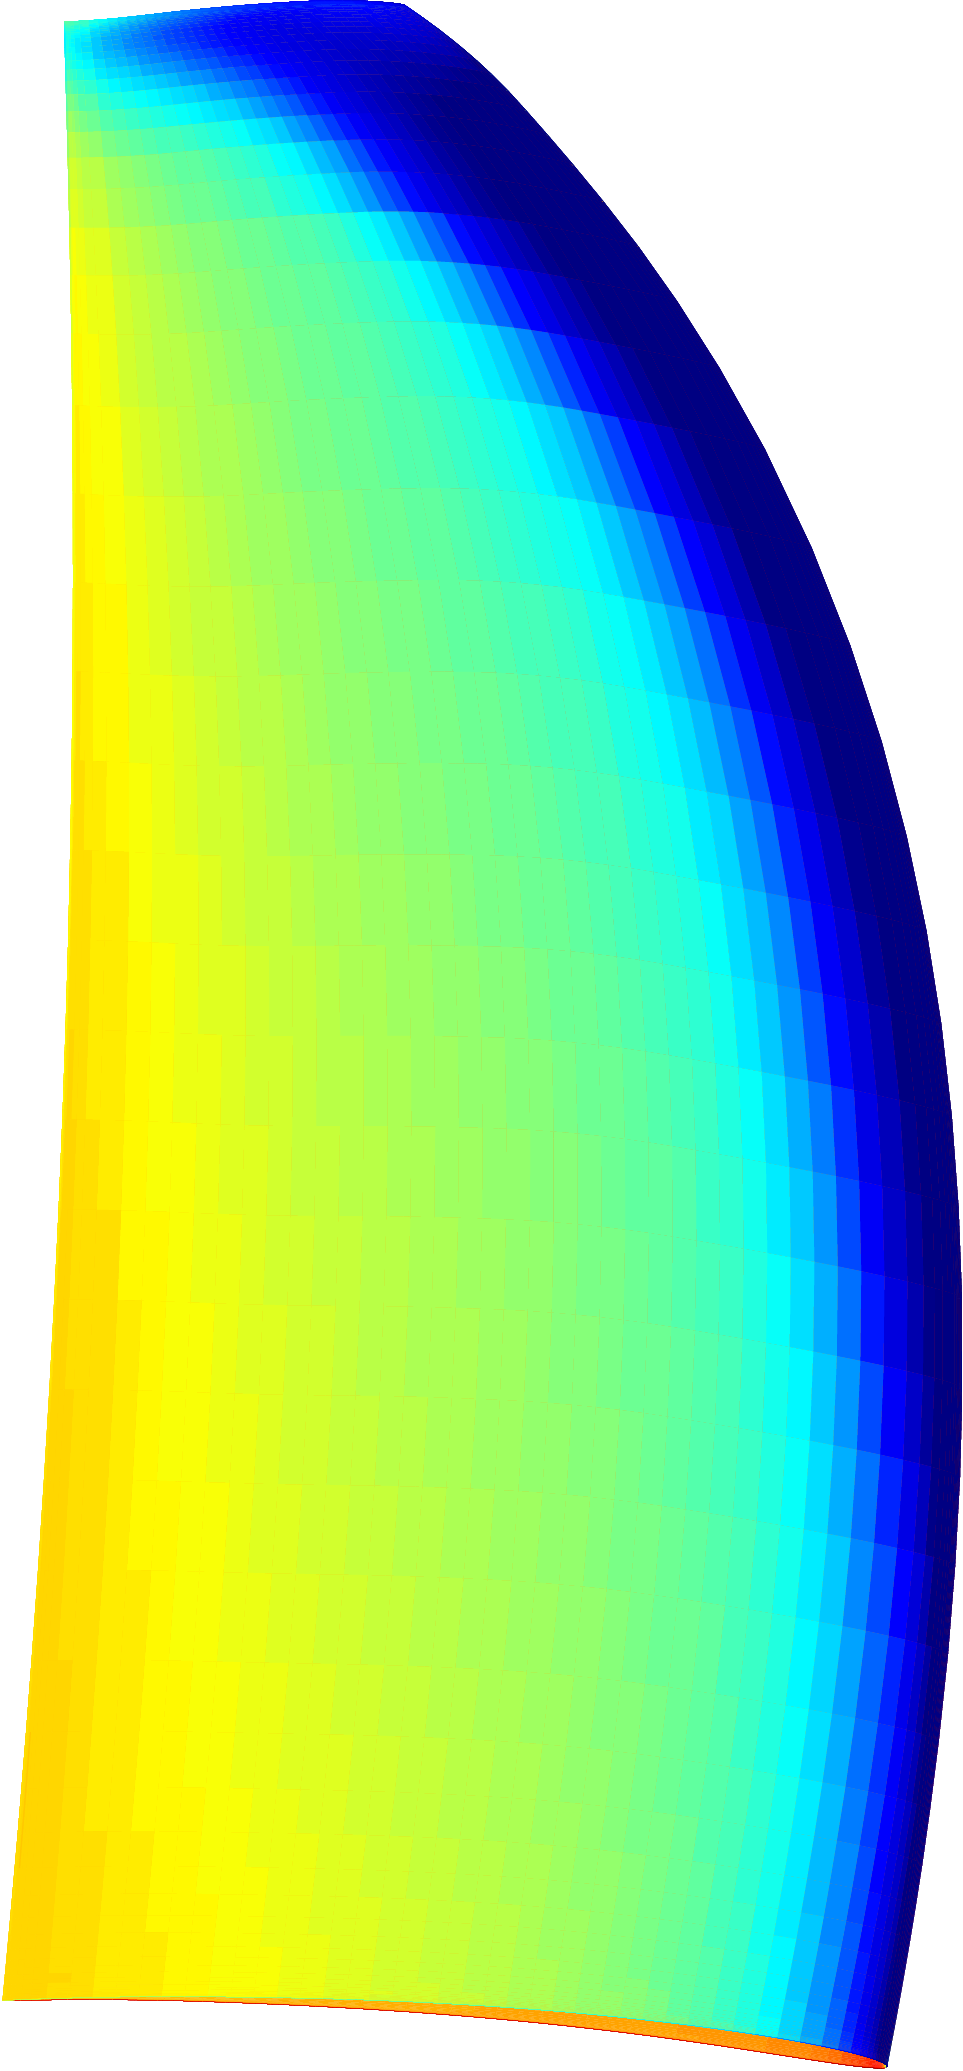
\includegraphics[width=0.10\textwidth]{DREAM_LS_TSM_N3_roe2_sa_blade_response_rear_mean_SS.png}
   & 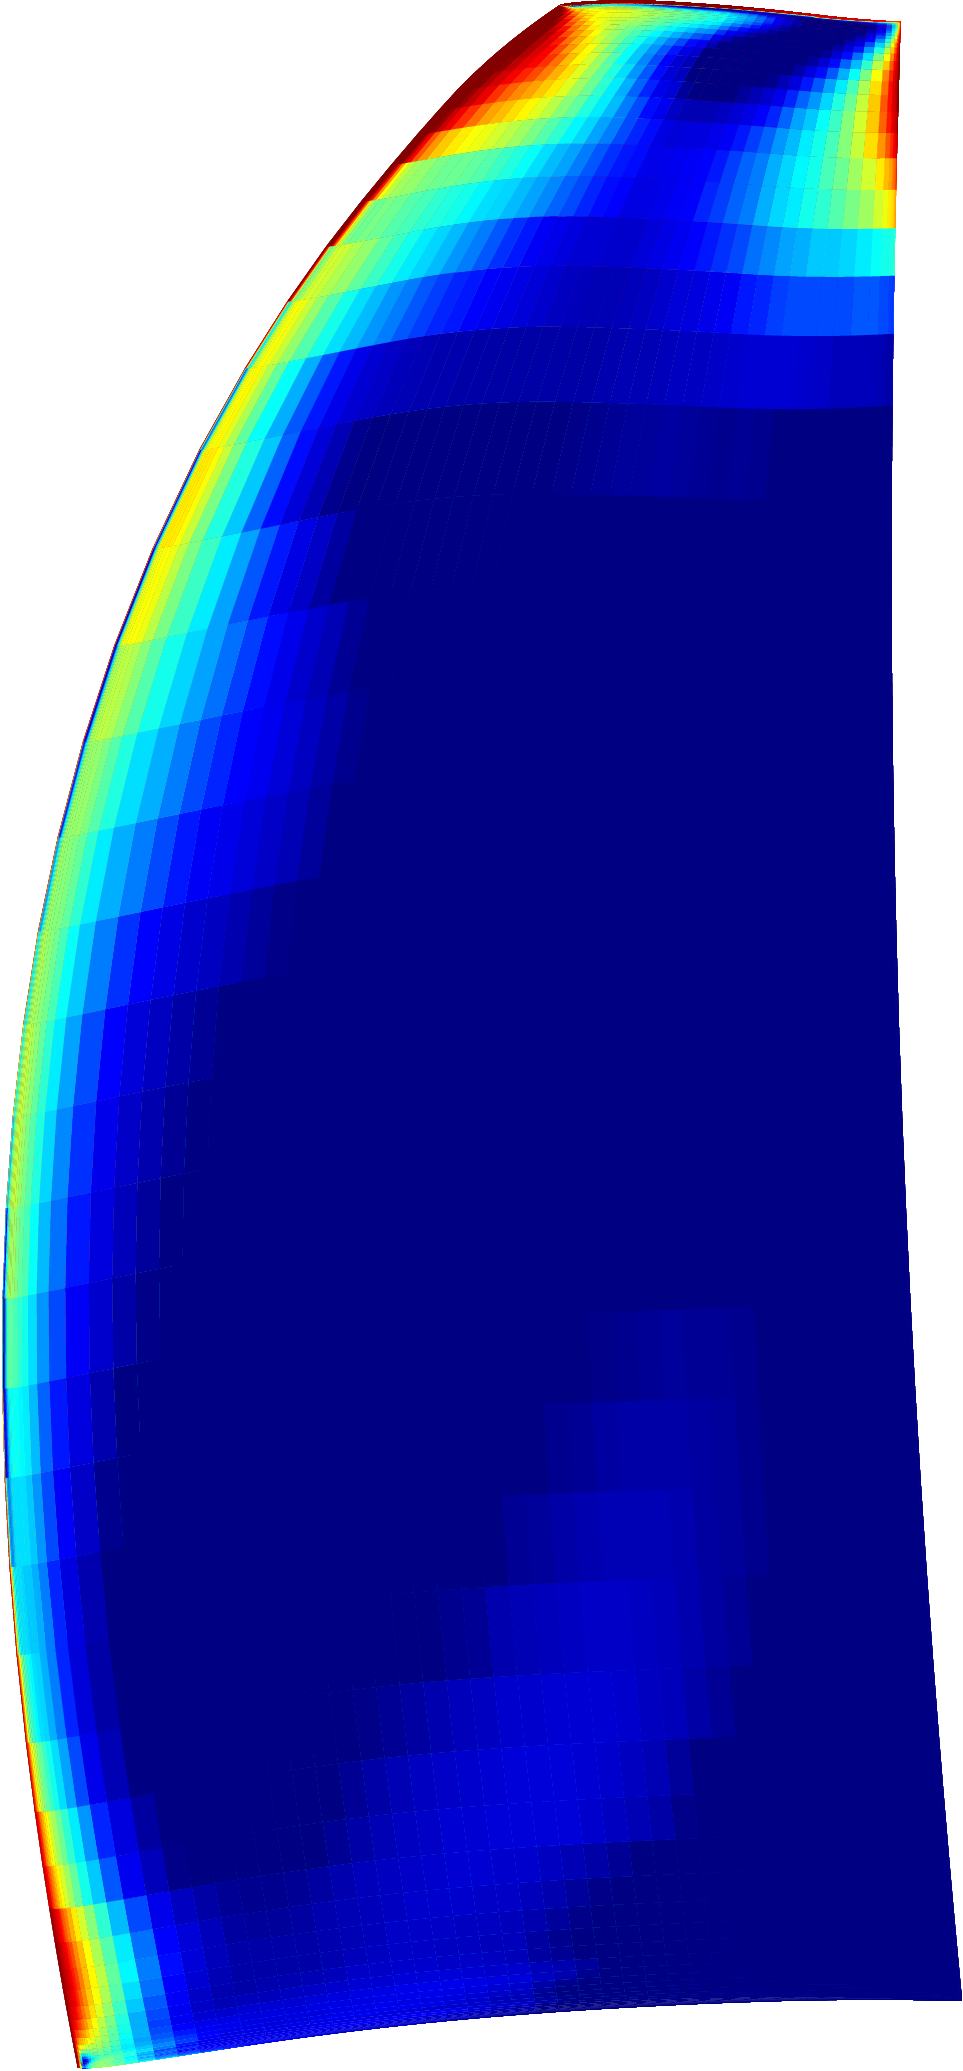
\includegraphics[width=0.10\textwidth]{DREAM_LS_TSM_N3_roe2_sa_blade_response_rear_H01_PS.png}
   & 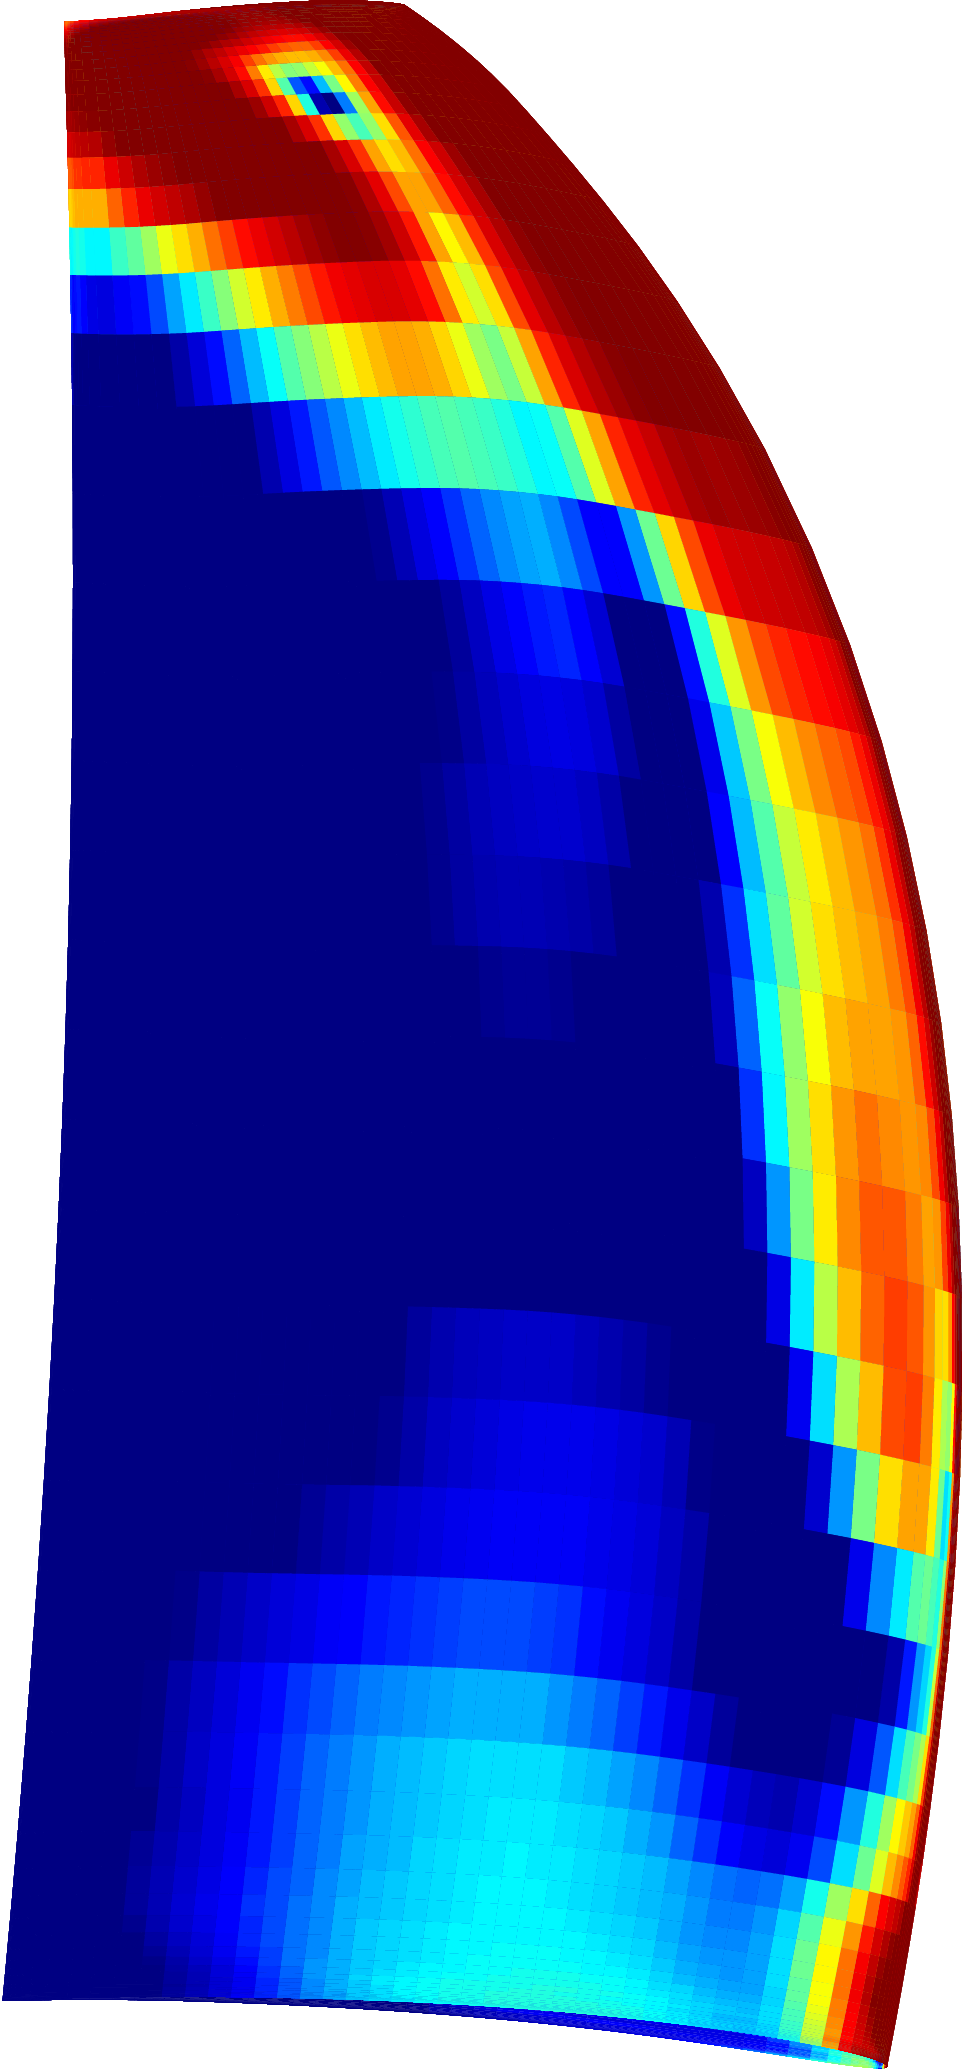
\includegraphics[width=0.10\textwidth]{DREAM_LS_TSM_N3_roe2_sa_blade_response_rear_H01_SS.png} \\
   \rotatebox{90}{\quad\quad HB $N=4$} 
   & 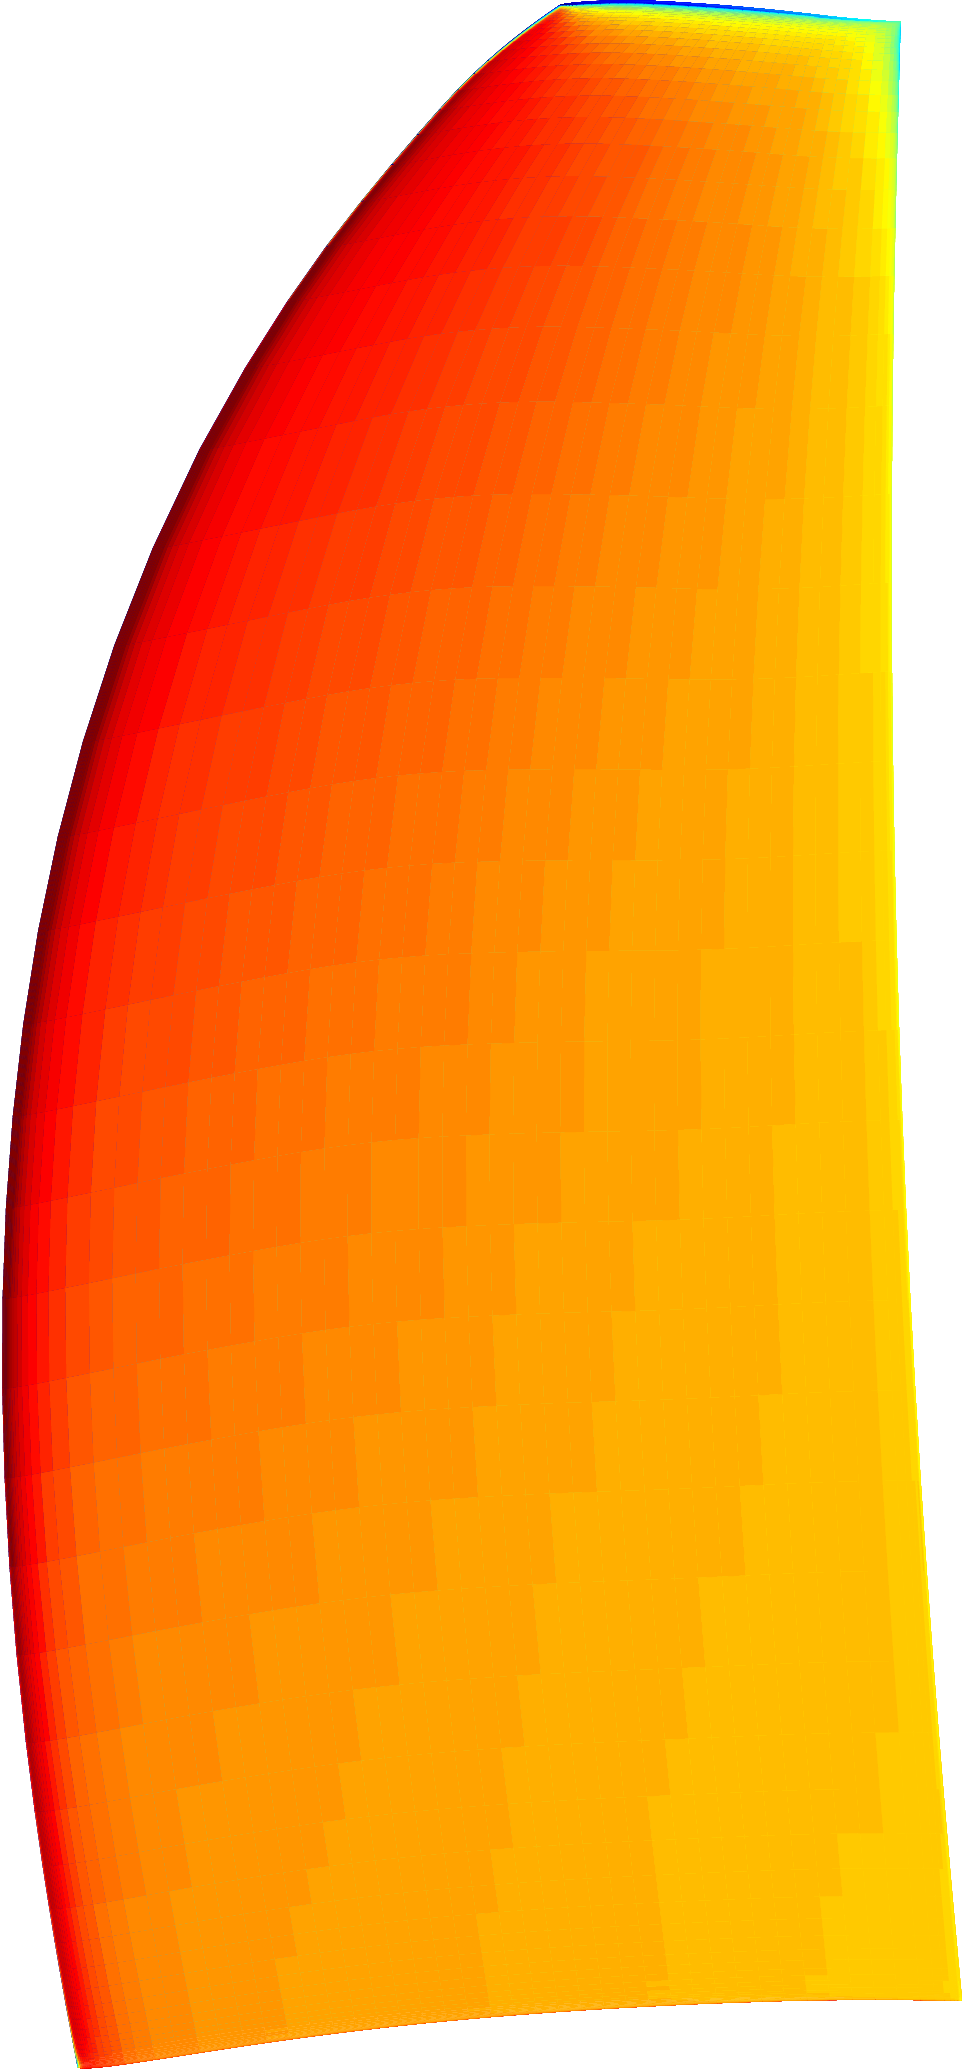
\includegraphics[width=0.10\textwidth]{DREAM_LS_TSM_N4_roe2_sa_blade_response_rear_mean_PS.png}
   & 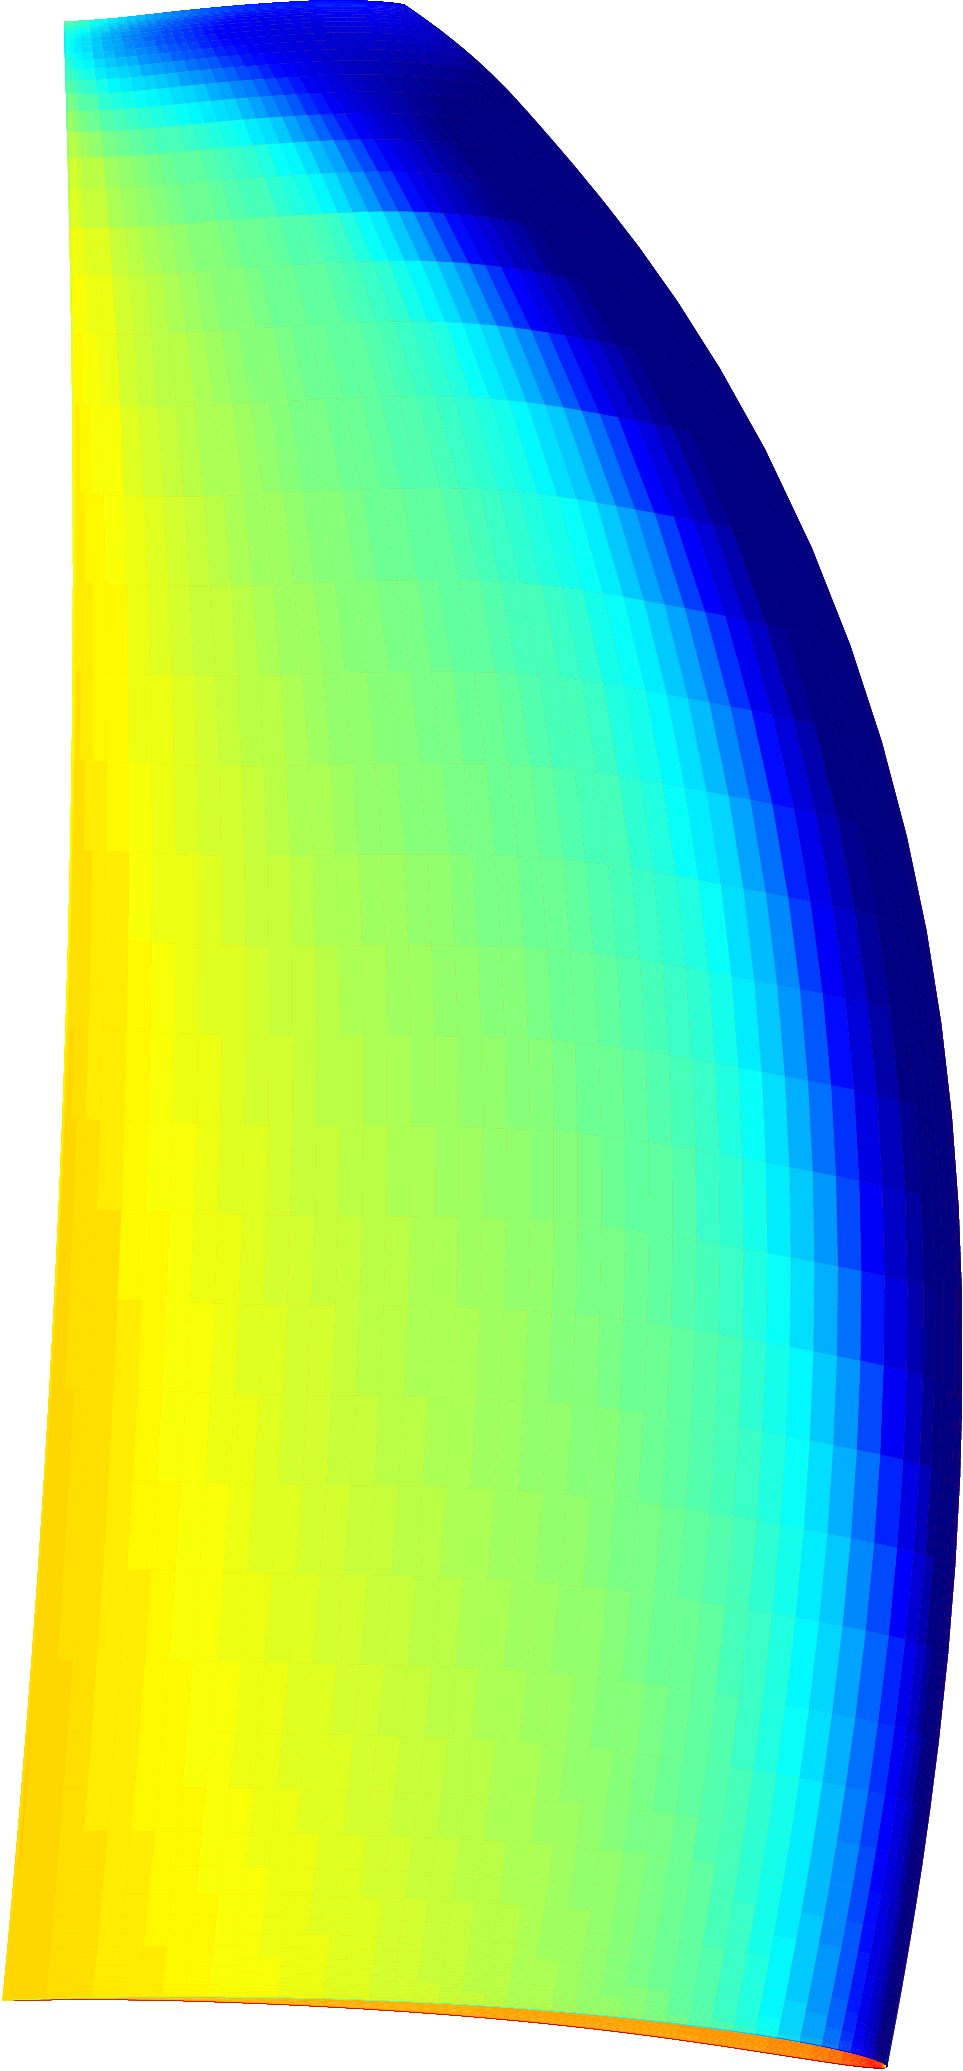
\includegraphics[width=0.10\textwidth]{DREAM_LS_TSM_N4_roe2_sa_blade_response_rear_mean_SS.png}
   & 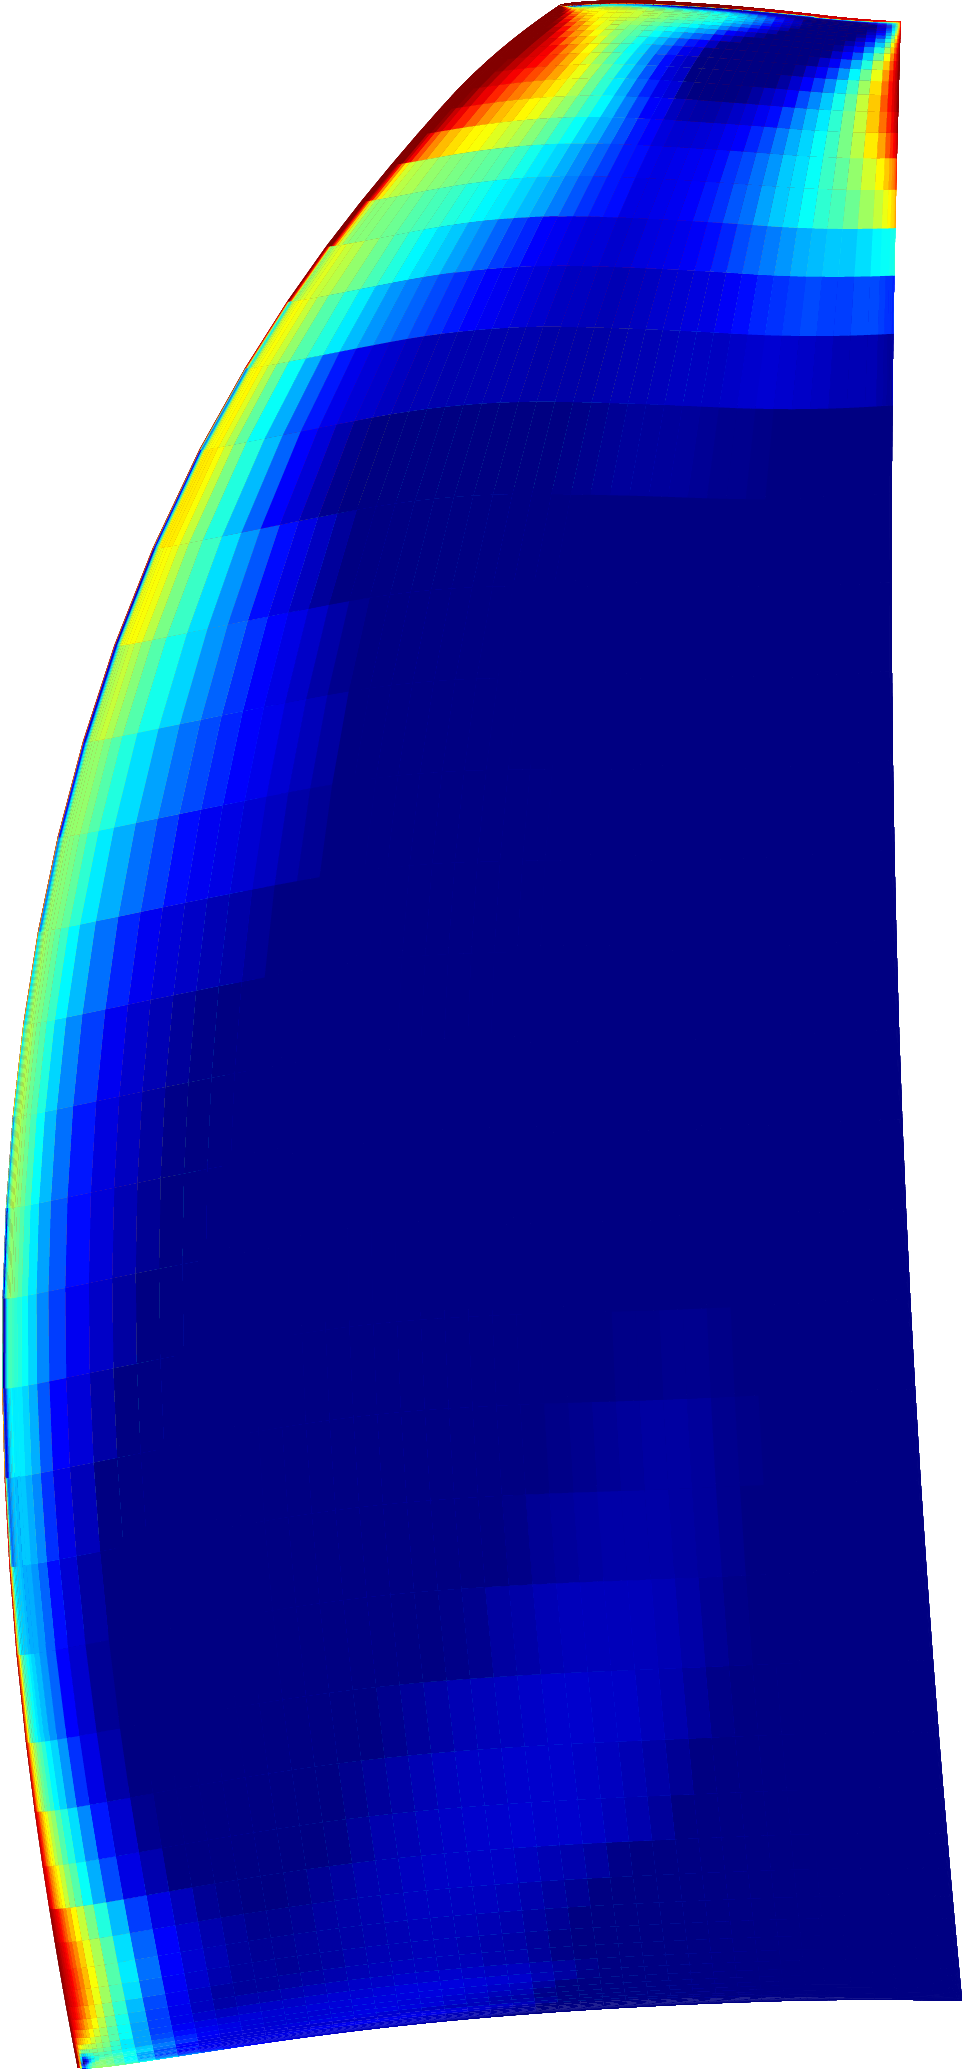
\includegraphics[width=0.10\textwidth]{DREAM_LS_TSM_N4_roe2_sa_blade_response_rear_H01_PS.png}
   & 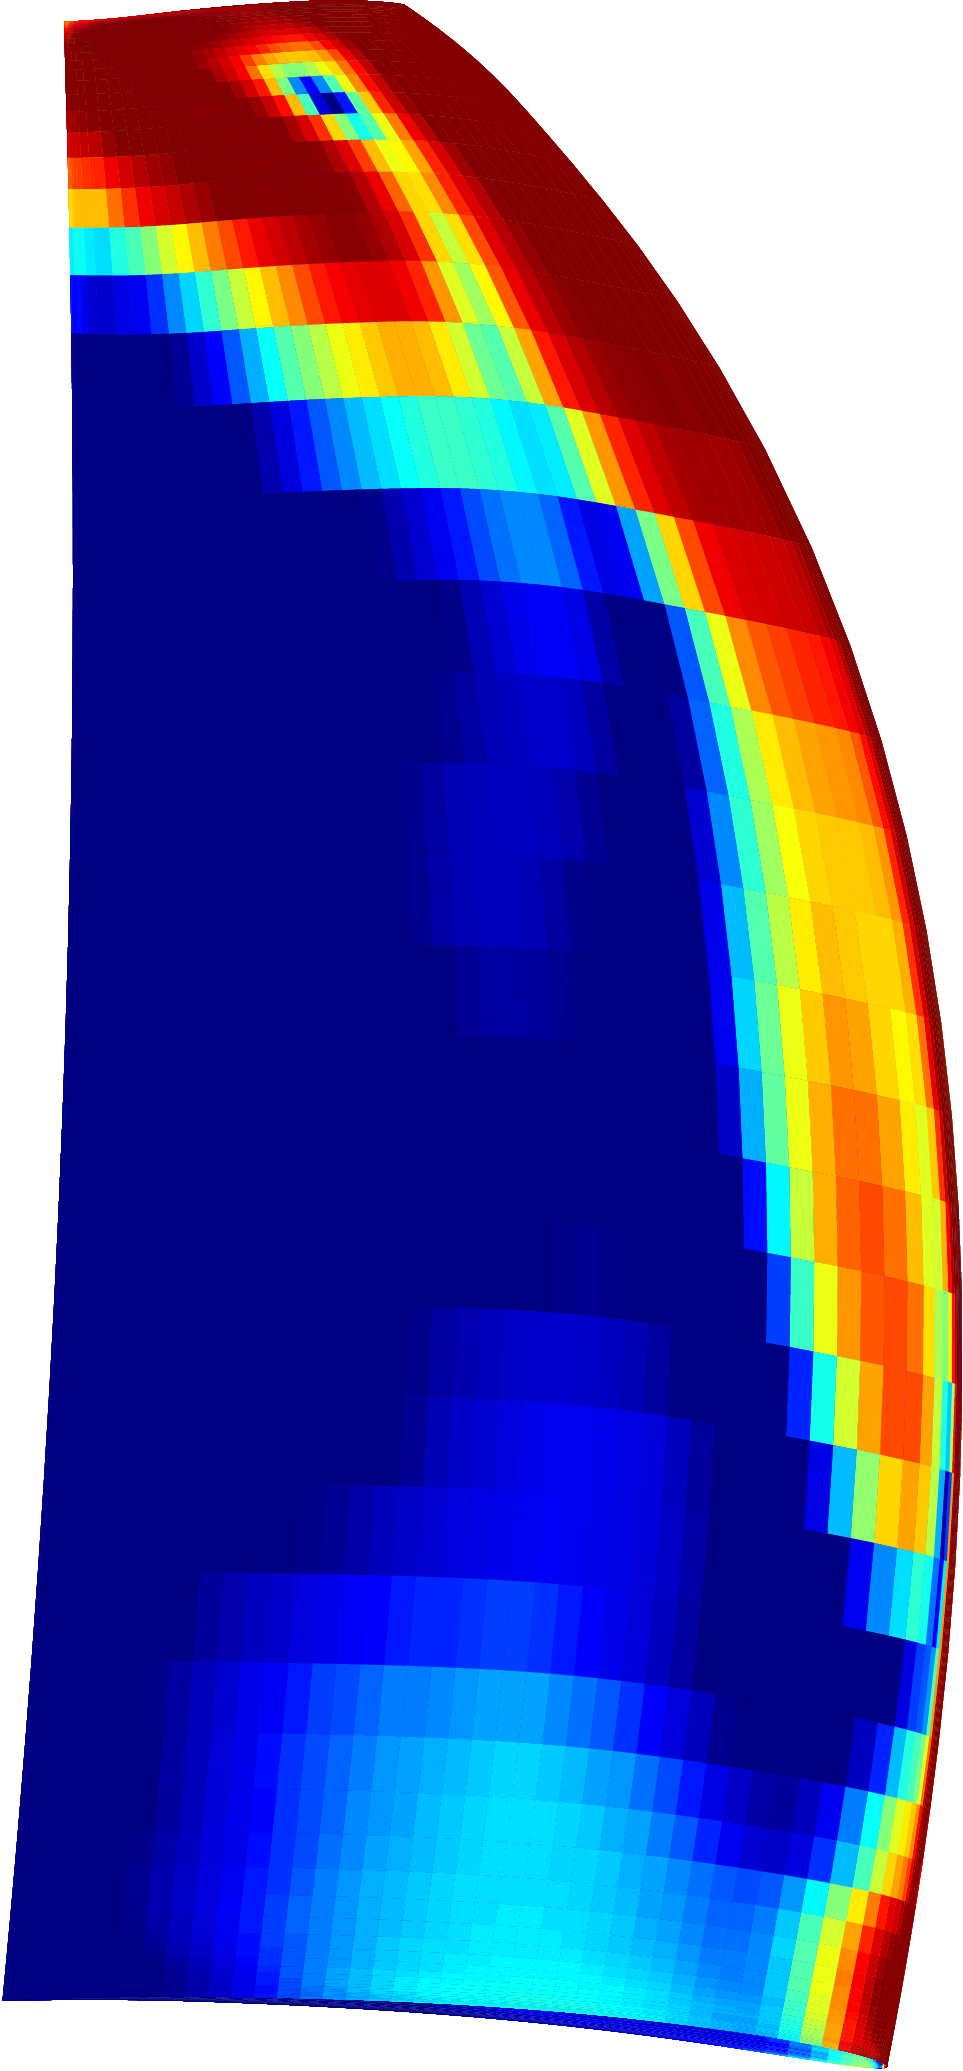
\includegraphics[width=0.10\textwidth]{DREAM_LS_TSM_N4_roe2_sa_blade_response_rear_H01_SS.png} \\
   \bottomrule
 \end{tabular}
 \caption{Low-speed isolated configuration: analysis of the number of harmonics
  required to capture the harmonic response of the rear rotor blades.}
 \label{fig:dream_ls_hb_blade_response_conv}
\end{figure}

Only one harmonic is needed to convergence the time-average value on the
rear rotor blades. Actually, the steady computation already gave a good prediction
of this time averaged value. This is due to the range on which this
low-speed CROR configuration operates. The Mach number is almost within the
incompressible range. As such, the non-linearities of the Navier--Stokes equations
remains small and steady approaches give good results.

Two to three harmonics are needed to converge the first harmonic 
pressure response on the rear rotor blade. This is a rough estimation
as a small convergence of the
harmonic pressure rise on the suction side of the blade between HB $N=2$, 
$N=3$ and $N=4$ computations can be seen. 

\subsection{Analyzing the radial cuts}
\label{sub:dream_ls_conv_hb_slice_r}
The final assessment of the convergence is done on radial cuts
of entropy made at 75\% of the height of the rear rotor blade. 
Remember that a propeller is supposed to be the most efficient at 75\% of the
blade (see Chapter~\ref{cha:cror}) which justifies the analysis done at this height.
The entropy spurious waves vanishes when computing the HB $N=4$ even though
the HB $N=3$ computation give a relatively smooth entropy field.
\begin{figure}[htp]
  \centering
  \subfigure[HB $N=1$]{
  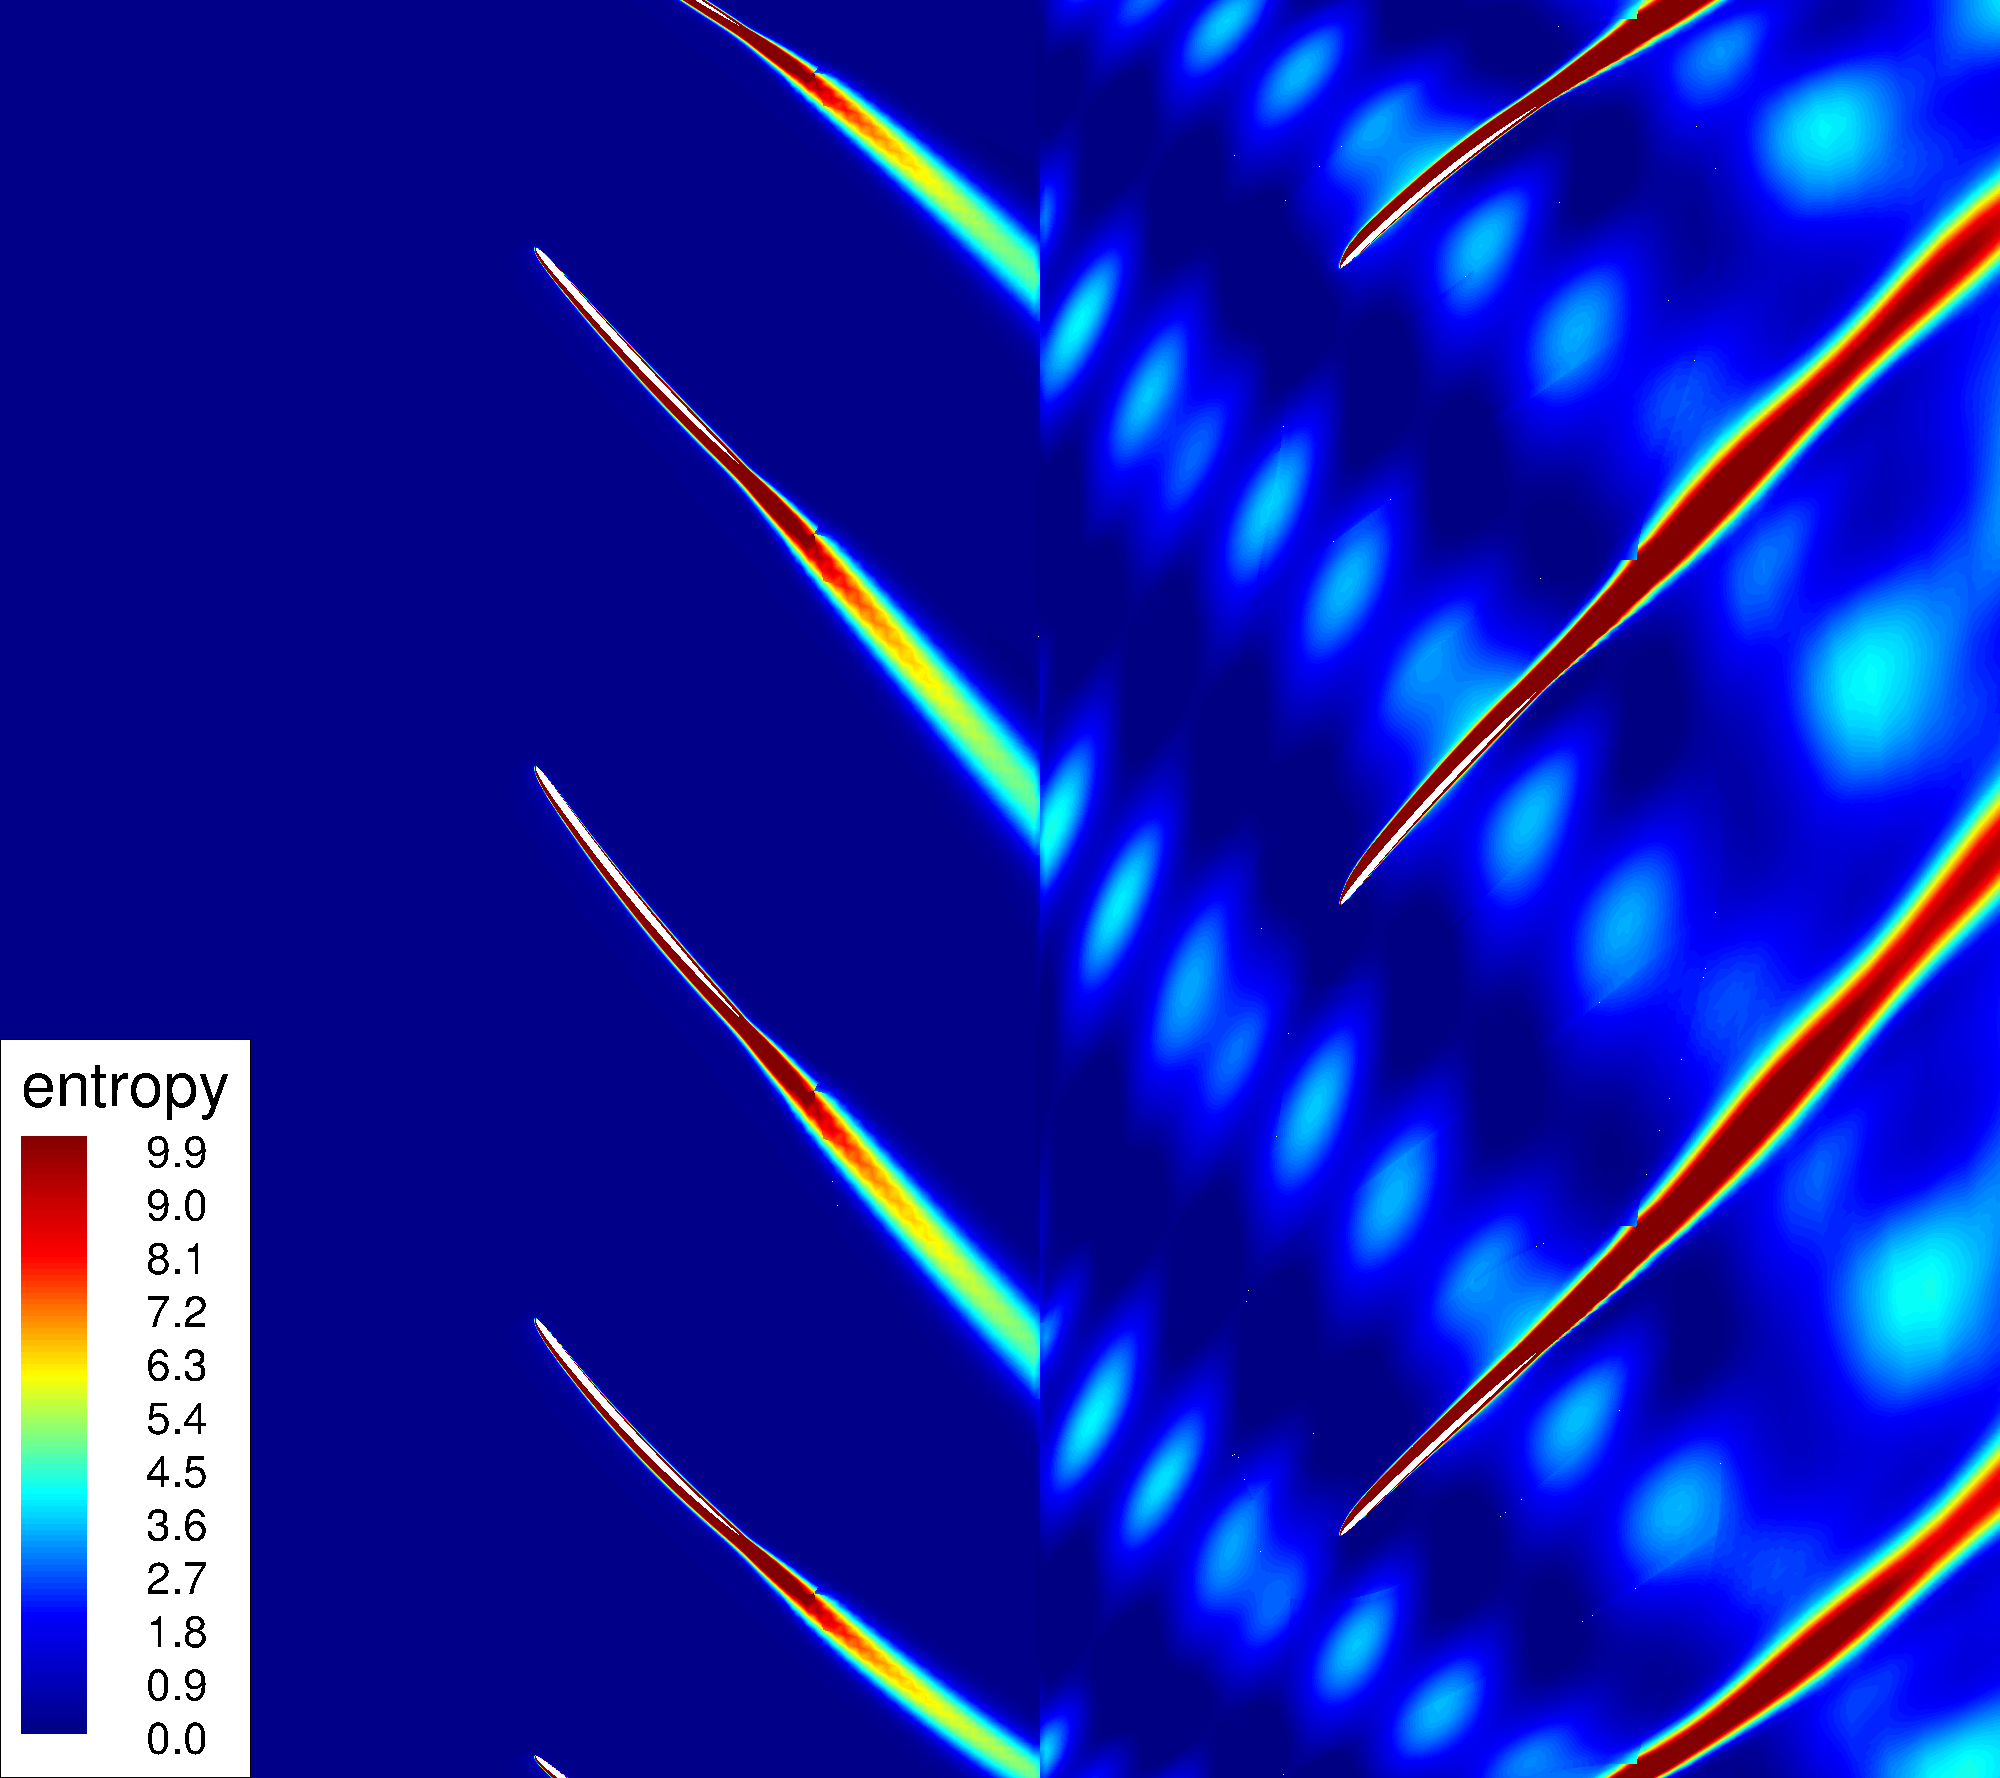
\includegraphics[width=.3\textwidth]{DREAM_LS_TSM_N1_roe2_sa_slice_r_75_entropy.png}}
  \subfigure[HB $N=2$]{
  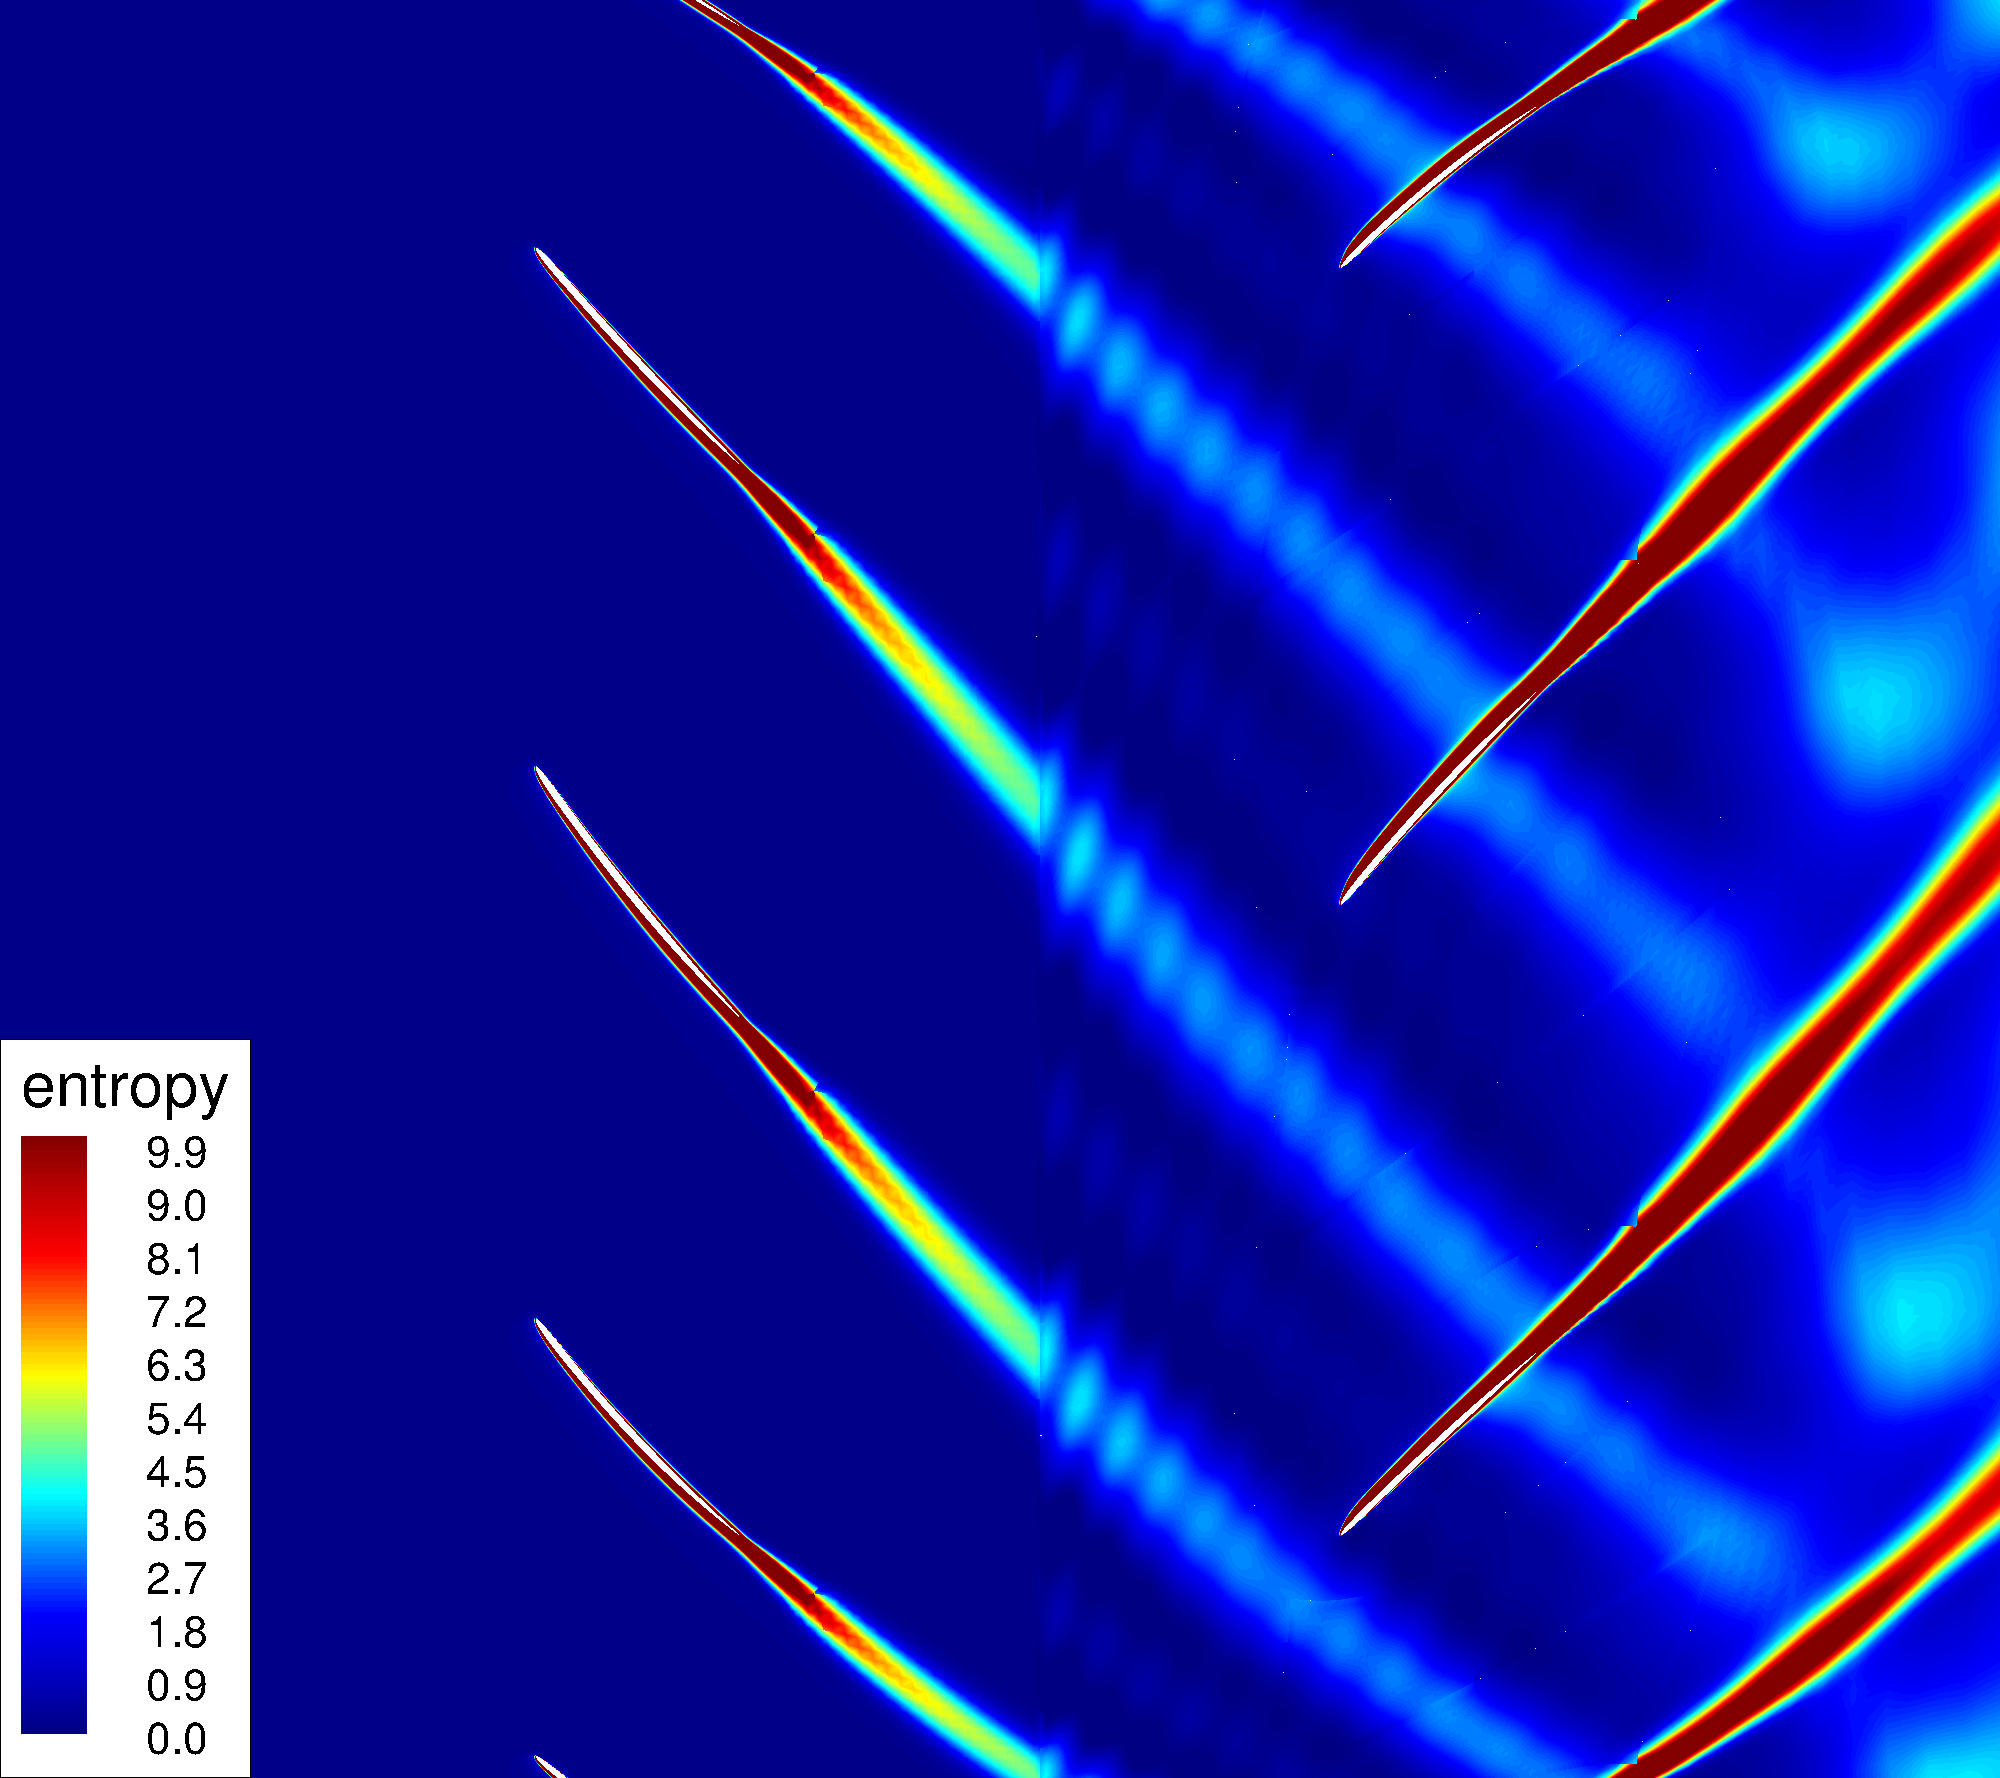
\includegraphics[width=.3\textwidth]{DREAM_LS_TSM_N2_roe2_sa_slice_r_75_entropy.png}}
  \subfigure[HB $N=3$]{
  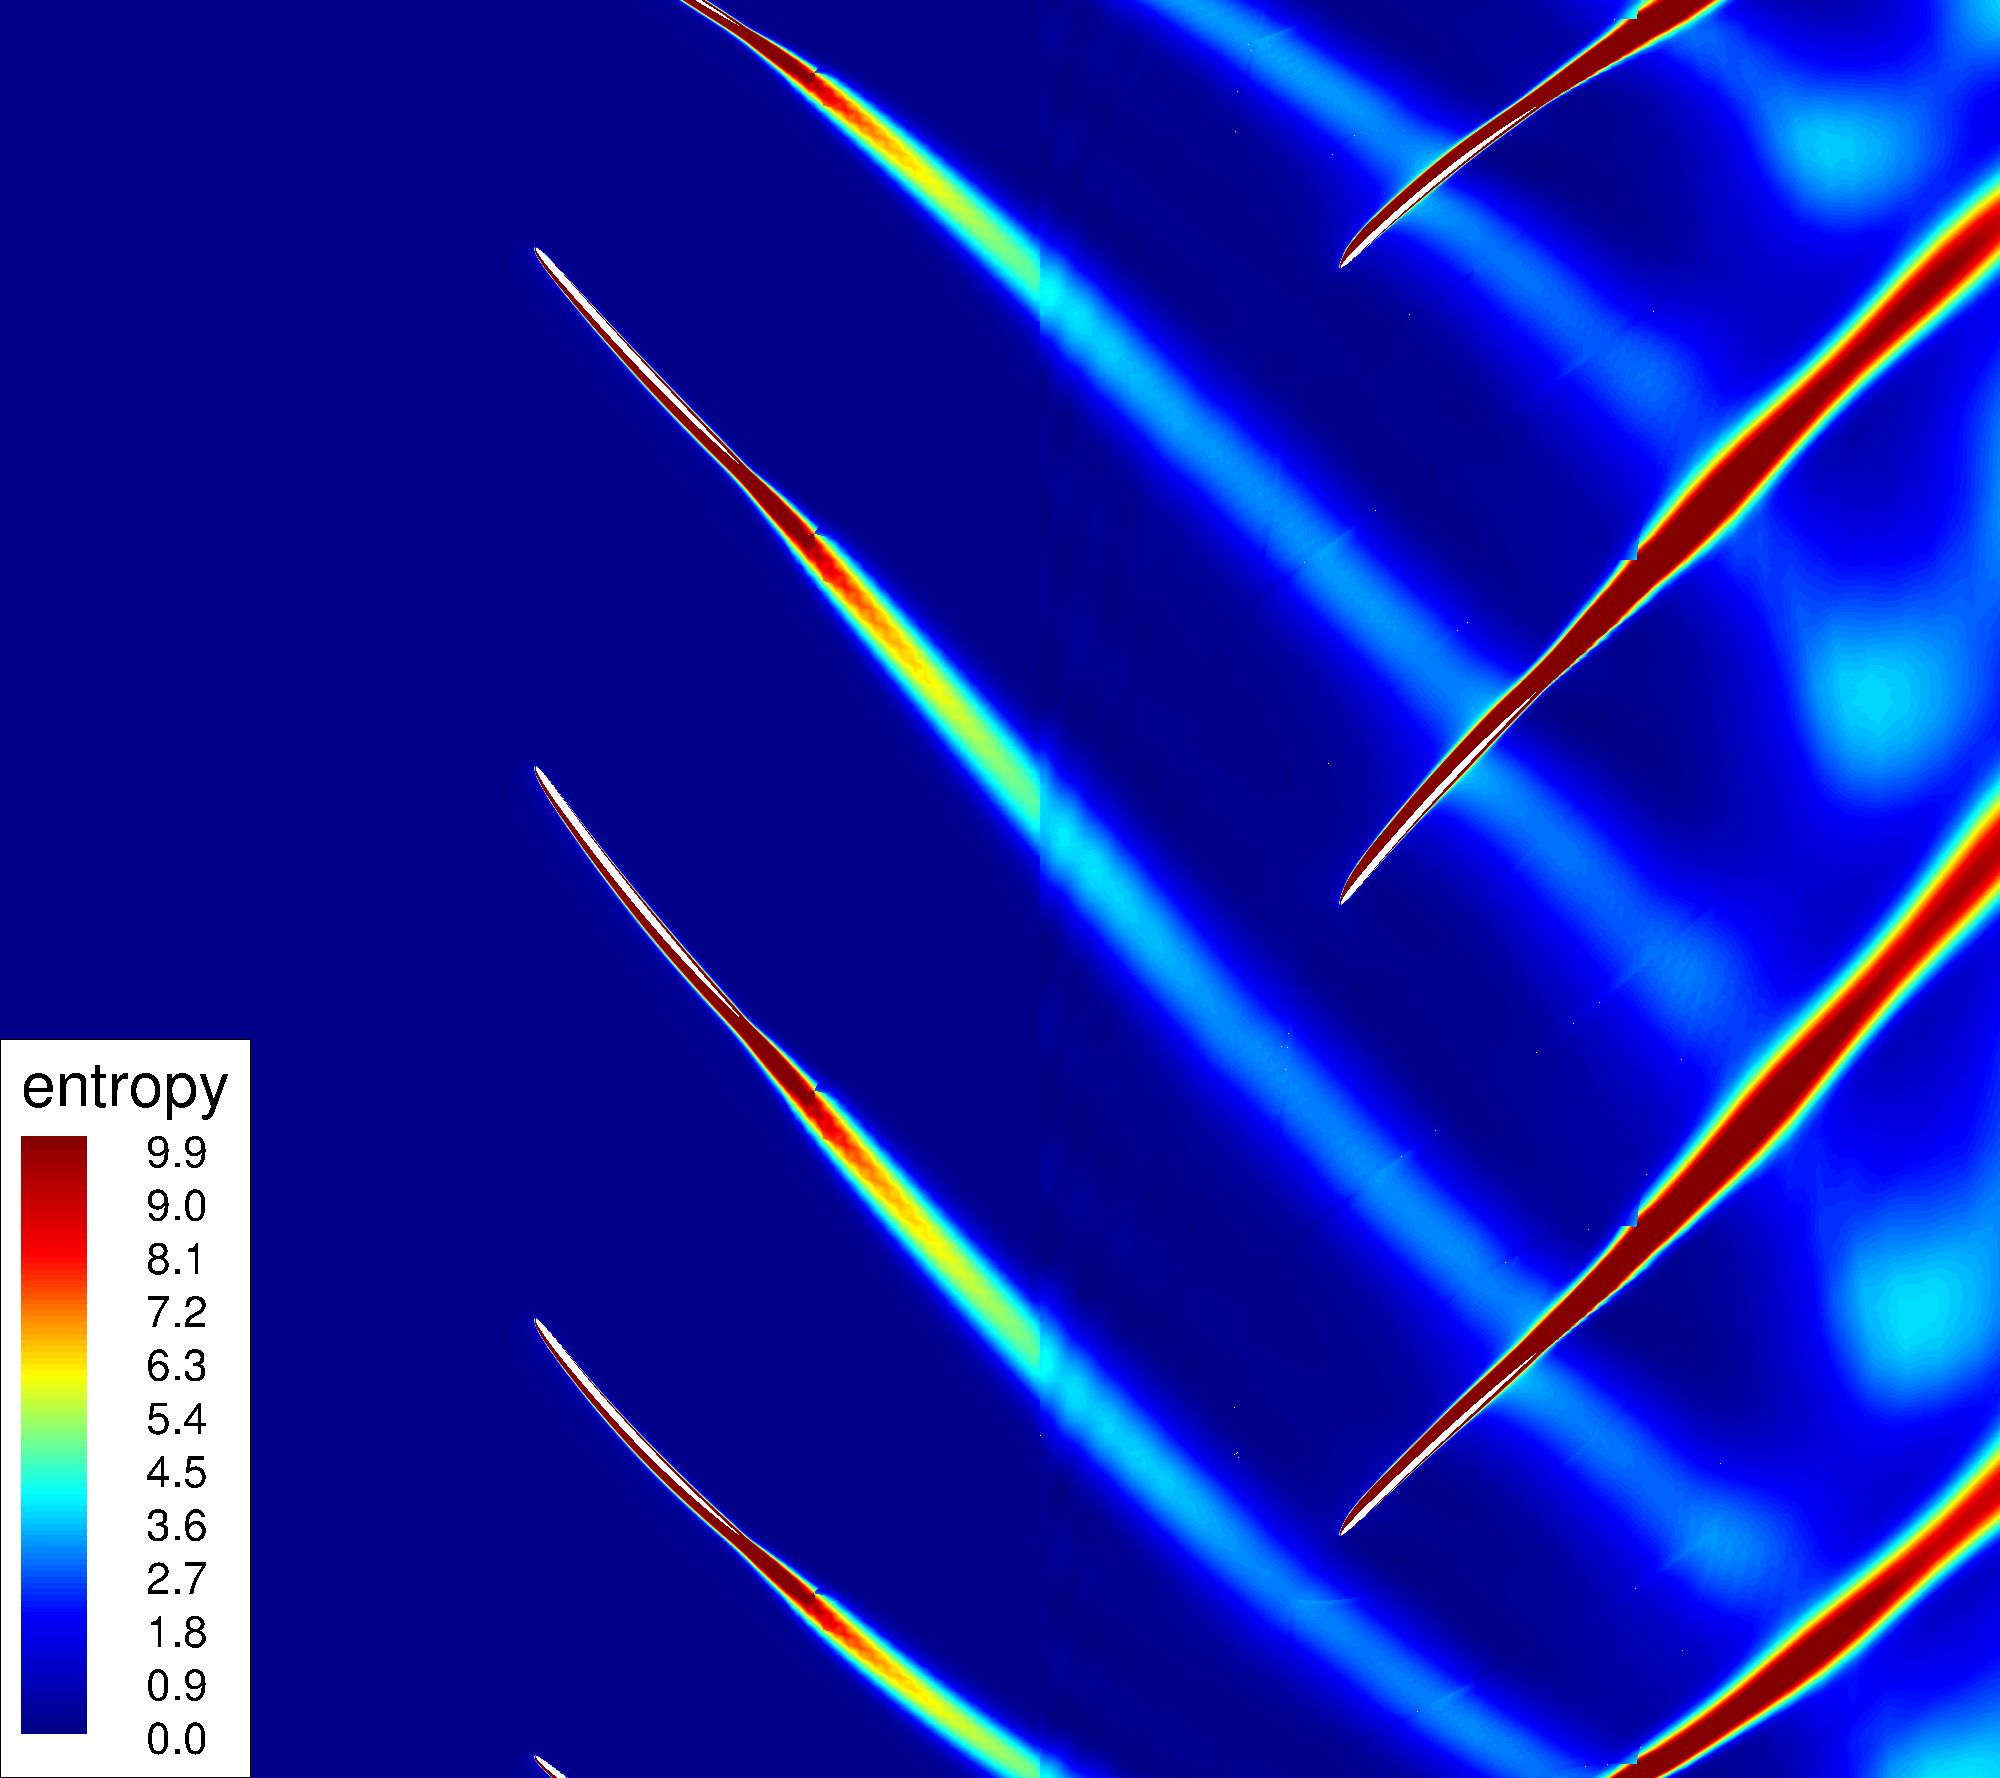
\includegraphics[width=.3\textwidth]{DREAM_LS_TSM_N3_roe2_sa_slice_r_75_entropy.png}}
  \subfigure[HB $N=4$]{
  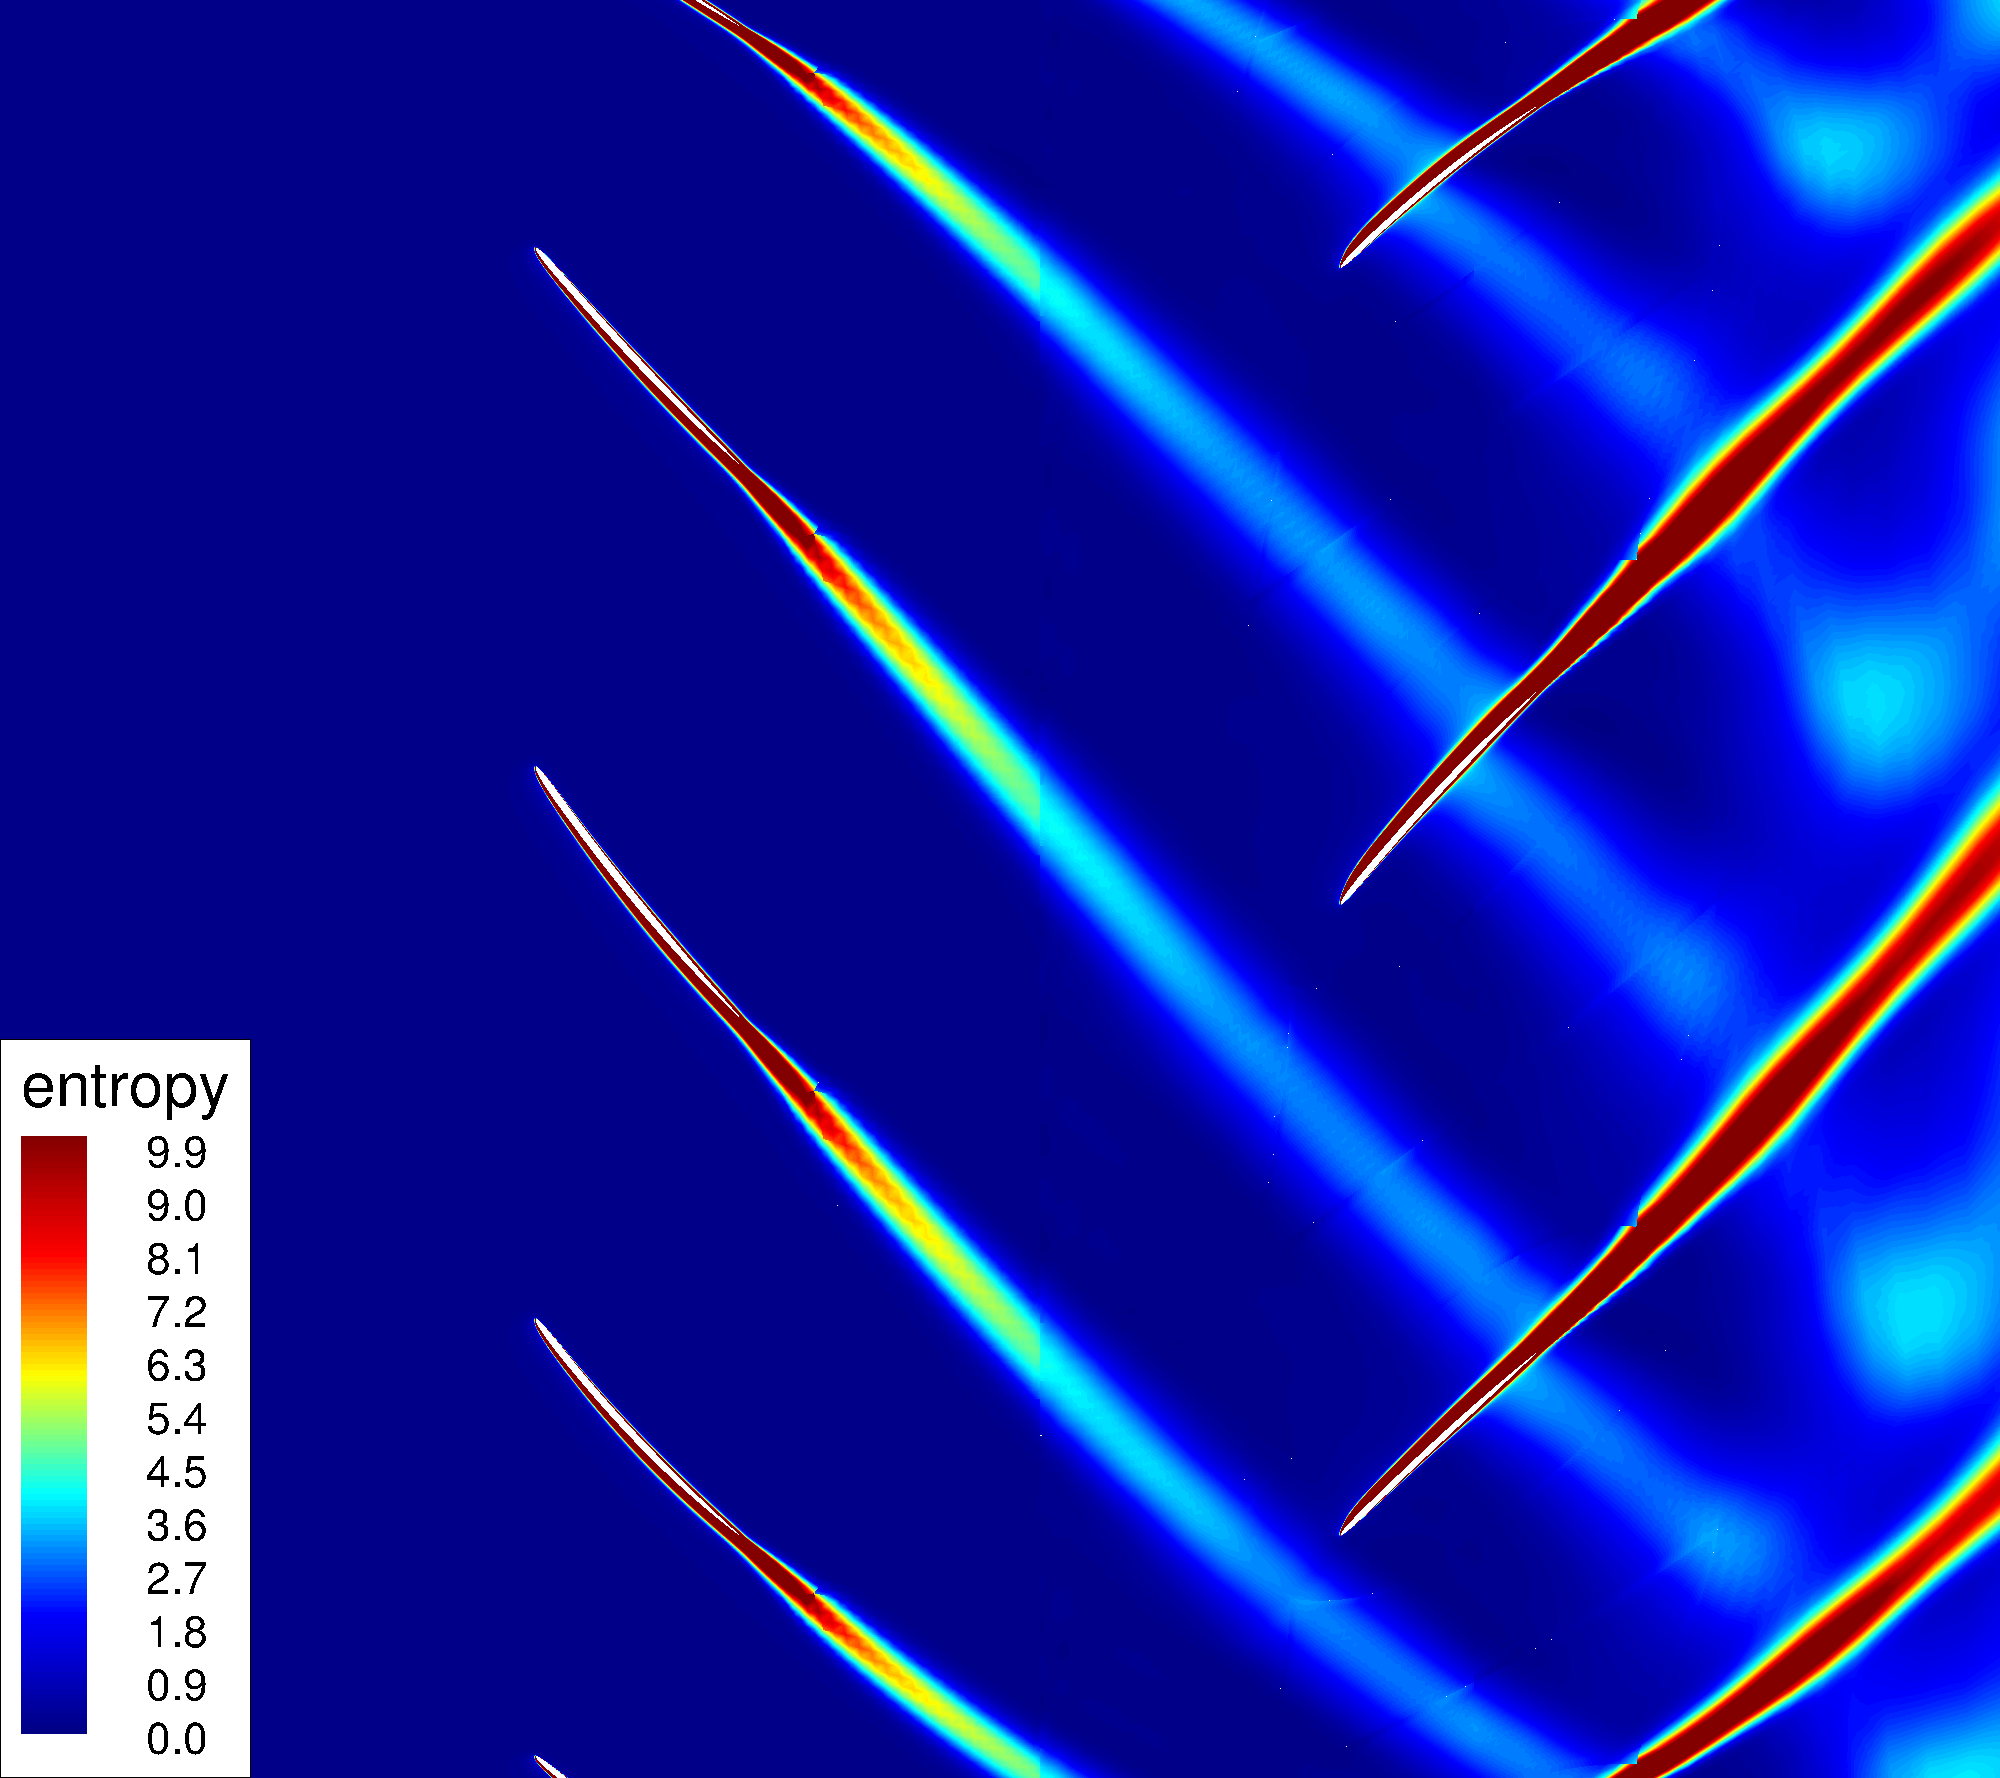
\includegraphics[width=.3\textwidth]{DREAM_LS_TSM_N4_roe2_sa_slice_r_75_entropy.png}}
  \caption{Low-speed isolated configuration: analysis of the number of harmonics
  required to capture the wake at a 75\% height radial cut.}
  \label{fig:dream_ls_hb_slice_r_conv}
\end{figure}
Nevertheless, the prediction tool, the
similarity coefficients, the harmonic blade response and the radial cuts give us confidence in
the HB $N=4$ computation. It is therefore chosen to further analyze the unsteady 
results on the HB $N=4$ computation.
